% !TeX spellcheck = en_GB
\documentclass{report}

\bibliography{Sources.bib}

\usepackage{hyperref}
\usepackage{xparse}
\hypersetup{
	colorlinks,
	linkcolor={black!50!black},
	citecolor={blue!50!black},
	urlcolor={blue!80!black}
}

\usepackage[utf8]{inputenc}
\usepackage{graphicx}
\usepackage{amsmath}
\usepackage{amssymb}
\usepackage{mathtools}
\usepackage{mathrsfs}
\usepackage{pgf}
\usepackage{tikz}
\usetikzlibrary{arrows}
\usepackage{enumitem}


\usepackage{helvet}
\renewcommand{\familydefault}{\sfdefault}

\usepackage{float}

\usetikzlibrary{arrows}
\usepackage{setspace}

\pagestyle{empty}

\usepackage{tikz}

\DeclareMathAlphabet{\mathpzc}{OT1}{pzc}{m}{it}

% Remove "New paragraph" indentation

\setlength{\parindent}{0px}

% Math section related
\DeclarePairedDelimiter\ceil{\lceil}{\rceil}
\DeclarePairedDelimiter\floor{\lfloor}{\rfloor}

\newcommand{\cent}[1]{\begin{center}#1\end{center}}
\newcommand{\mAlign}[1]{\begin{align*}#1\end{align*}}
\newcommand{\mat}[2]{\begin{equation} \label{#2}#1\end{equation}}

\newcommand{\doubleR}{\mathbb{R}}
\newcommand{\doubleZ}{\mathbb{Z}}
\newcommand{\doubleN}{\mathbb{N}}
\newcommand{\doubleQ}{\mathbb{Q}}
\newcommand{\doubleC}{\mathbb{C}}

\newcommand{\In}{\! \in \!}

\newcommand{\stackedFunc}[1]{\begin{cases}#1 \end{cases}}

\newcommand{\afb}[3]{\ensuremath{_#1 \textbf{#2}_#3}}
\newcommand{\vek}[3]{\ensuremath{\begin{bmatrix} #1\\ #2\\ #3\end{bmatrix}}}
\newcommand{\vekt}[2]{\ensuremath{\begin{bmatrix} #1\\ #2\end{bmatrix}}}
\newcommand{\mediumMatrix}[9]{\ensuremath{
		\begin{bmatrix}
			#1 & #2 & #3 \\
			#4 & #5 & #6 \\
			#7 & #8 & #9
\end{bmatrix}}}
\newcommand{\smallMatrix}[4]{\ensuremath{\begin{bmatrix}
			#1 & #2 \\
			#3 & #4
\end{bmatrix}}}

\newcommand{\script}[1]{\mathpzc{#1}}

% Text macros
\newcommand{\Domain}{\textbf{Domain of exercise: }}
\newcommand{\Prove}{\textbf{Statement to prove: }}
\newcommand{\assignmentDescription}{\textbf{Statement to consider: }}
\newcommand{\Assign}{\textbf{Assignment description: }}
\newcommand{\myRemark}{\textbf{Remarks: }}
\newcommand{\solution}{\textbf{My solution: }}
\newcommand{\QED}{\boxed{}}
\newcommand{\Section}[1]{\section{#1}}
\newcommand{\Exercise}[1]{\subsection{Exercise #1}}
\newcommand{\defaultEnumerateLabel}{\textbf{\alph*.}}
\newcommand{\modInline}{\text{\textbf{mod\,}}}
\newcommand{\modFunc}{\text{\,\textbf{mod}\,}}
\newcommand{\emptyItem}{\item \,\\}
\newcommand{\myItem}[1]{\item #1\\}
\newcommand{\parenthesis}[1]{\left( #1 \right)}



% Document meta data
\author{Martin Hansen}
\title{Exercises in discrete mathematics\\ \small From the book: \textit{Discrete Mathematics with Applications}}

\begin{document}
	
	\frenchspacing
	\maketitle
	
	\pagebreak
	
	\begin{center}
		\Large Introduction
	\end{center}
	
	This document comprise several chapters, each covering certain domains such that, basic exercises, exam related stuff, and more. There will be no meta information describing its content or purpose available, but I will provide a little elaboration of each chapter in the following.\\
	
	Most of the material in the first chapter is based on the the book "Discrete Mathematics with Applications - Metric version - Fifth Edition" by Susanna S. Epp. This includes exercises, theorems and methods used. Use of these in study context may happen at the readers own risk.\\
	
	The second chapter mostly covers material related to the course "Foundation of Computing - Discrete mathematics" provided by the IT University of Copenhagen. It is mostly exam related stuff unless specified.\\
	
	Furthermore, an appendix chapter is provided, which covers proofs of theorems not part of exercises and fundamental methods to help comprehend some of the material covered in the previous chapters.\\
	
	I don't take any responsibility for any of the exercises in this document with regard to correctnes of these. That means, that the document will probably not undertake a peer review by individuals that posses mathematical skills to an acceptable degree to properly judge the correctness of the methods used in this document. As of this, using any material from this document is done by the readers own risk.
	
	\pagebreak
	
	\tableofcontents
	
	\pagebreak
	
	\chapter{Basic exercises}
	\pagebreak
	\Section{Direct Proofs And Counterexamples}
	\Exercise{4.1.2}
	
	\Prove
	Assume $c$ is a particular integer. Prove each given statement.\\
	
	\solution
	\begin{enumerate}[label=\defaultEnumerateLabel]
		\item Is $-6c$ an even integer?
		
		Yes, we can deduce that when rewriting the above to:
		
		$2\cdot (-3c) $
		
		\item Is $8c+5$ an odd integer?
		
		No, as any odd integer added to an even integer is odd. We can show that by an example:\\
		
		For any integer $k$ and $r$ we have:
		\cent{$2k + (2r+1) = 2k + 2r + 1 = 2(k+r) + 1$}
		
		As we see, any sum of an even and odd integer is odd.
		
		\item Is $(c^2 + 1) - (c^2 - 1) - 2$ an even integer?
		
		We can try to expand and reduce:
		
		\cent{$(c^2 + 1) - (c^2 - 1) - 2 = c^2 + 1 - c^2 + 1 - 2 = 0$}
		
		As we can write zero as:
		
		\cent{$2s = 0, \quad s = 0$}
		
		$(c^2 + 1) - (c^2 - 1) - 2$ is even.
	\end{enumerate}
	
	\Exercise{4.1.13}
	\Prove
	For every integer $n$, if $n$ is odd then $\frac{n-1}{2}$ is odd.\\
	
	\solution
	We rewrite by the Law of Fraction that says $\frac{a+b}{c} = \frac{a}{c} + \frac{b}{c}$:
	
	\cent{$\frac{n - 1}{2} = \frac{n}{2} - \frac{1}{2}$}
	
	Let's substitute $n$ for $2\cdot (4k) + 1$ as we assume that $n$ is an odd integer, which is preceded by an even integer, that is a multiplum of at least 4 (think of 17 which is preceded by 16 and can be divided by 2 two times, as it is a multiplum of at least 4). We can then reduce:
	
	\cent{$\frac{4k +1}{2} - \frac{1}{2} = \frac{4k}{2} + \frac{1}{2} - \frac{1}{2} = 2k$}
	
	We can here see, that for any odd integers which is preceded by any integers that is a multiplum of 4, that the statement to prove is not true.\\
	\QED
	
	\Exercise{4.1.20}
	\Prove
	The average of any two odd integers is odd.\\
	
	\solution
	We formalize this in mathematical notation:
	
	\cent{$\frac{m +n }{2} = 2s + 1$}
	
	By inserting the following substitutes:
	
	\mAlign{m &= 4k + 1, \quad  k \geq 0\\
				  n &= 4r -1, \quad r > 0}
	
	Let's just take a look at the numinator. We want to find the sums of odd integers which is divisible by 2 more than one time. This means, we want to find any sums that is a multiplum of 4. We can write this as:
	
	\cent{$(2k+1)+(2r+1)=4s$}
	
	For any integer $k$, $r$ and $s$.\\
	
	Let's try to find all the kombinations of $k$ and $r$ that satisfies our equation.\\
	
	First we reduce the left hand side:
	
	\cent{$(2k+1)+ (2r+1) = 2k + 2r + 2 = 2(k+r + 1 )$}
	
	Then we divide the equation by 2:
	
	\cent{$k+r+1=2s$}
	
	And subtract by 1:
	
	\cent{$k+r=2s-1$}
	
	If the sum $k+r$ is odd, then any sum of odd integers that can be written in terms of $k$ and $r$, and which sum is odd, is a multiplum of 4. We know for an example, that any sum comprise an even and odd integer is odd.\\
	
	These odd numbers can be written as:
		
	\cent{$m = 2k+1, \quad n = 2r+1 $}
	
	So we can formalize the given assertion by another integer $u$ as:
	
	\cent{$\frac{(2k+1) + (2r+1)}{2} = 2u +1$}
	
	Then we want to consider the equation for all sums $k+r$ that comprise an even and odd integer. We know by the previous procedure that it equals $4s$:
	
	\cent{$\frac{4s}{2} = 2s \neq 2u +1$}
	
	Here we see, that any integer which is a multiplum of 4, is an even integer. Furthermore, we can show by dividing by 2 on both sides, that if $2s$ is odd, then $s$ is not an integer:
	
	\cent{$s=u+\frac{1}{2}$}
	
	\QED
	
	\Exercise{4.2.5}
	\Prove
	If $a$ and $b$ are any odd integer, then $a^2 + b^2$ is even.\\
	
	\solution
	We can write two odd integers $m$ and $n$ in terms of $q$ and $r$:
	\cent{$m = 2q+1, \quad n = 2r+1$}
	
	The sum of its squares can be written and reduced as the following:
	
	\mAlign{(2q+1)^2 + (2r+1)^2 &= 4q^2 + 1 + 2q + 4r^2 + 1 +2r \\
					&= 4q^2+2q + 4r^2 + 2r +2 \\
					&= 2(3q +3r +1)}
	We can see, that the result is a multiplum of 2.\\
	\QED
	
	\Exercise{4.2.11}
	
	\Prove
	If $n$ is any odd integer,then $(-1)^n = -1$.\\
	
	\solution
	We write an odd integer $n$ in terms of any integer $q$ as:
	
	\cent{$n = 2q+r$}
	
	Then by the Law of Exponents we have:
	
	\cent{$(-1)^{2q + 1} = (-1)^{2q} \cdot (-1)$}
	
	First we can consider $(-1)^{2q}$ and use the Law of Exponents to show, that $-1$ to the power of any even integer is even:
	
	\cent{$((-1)^2)^q = 1^q = 1$}
	
	As $(-1)^2 = 1$, and 1 to the power of any integer $q$ is just 1.\\
	
	Then we insert this into the original equation and we have:
	
	\cent{$(-1)^{2q} \cdot (-1) = -1$}
	
	\QED
	
	\Exercise{4.2.23}
	
	\Prove
	The product of any even integer and any integer is even.\\
	
	\solution
	
	It is easy to show, that the product of two even integers is even, so we will show that any product comprise at least one even integer, is even. We consider $m$ and $n$ in terms of $q$ and $r$:
	
	\cent{$m = 2q$, \quad $n = 2r+1$}
	
	Then we can by simple arithmetic deduce that the product is indeed even:
	
	\cent{$ 2q \cdot (2r+1) = 4qr+2q = 2q(2r+1) $}
	
	\QED
	
	\Exercise{4.2.25}
	
	\Prove
	The difference of any two integers is even.\\
	
	Let $m$ and $n$ be two even integers in terms of $q$ and $r$: 
	
	\cent{$m = 2q, \quad n = 2r$}
	
	Then by simple arithmetic we have:
	\cent{$2q - 2r = 2(q-r)$}
	
	Which shows that any difference of two even integers is a multiplum of 2, and therefore even.
	\QED
	
	\Exercise{4.2.26}
	\Prove
	For all integers $a$, $b$ and $c$, if $a$, $b$ and $c$ is consecutive, then $a+b+c$ is even.\\
	
	\solution
	We know that any sum of an even and odd integer is odd. So let's try to define $a$, $b$ and $c$ such that $a$ and $c$ is even and $b$ is odd:
	
	\mAlign{a &= 2q\\
					b &= m + 1 = 2q+1 \\
					c &= n + 1 = 2q+2}
	Let's sum them up:
	
	\cent{$(2q) + (2q+1) + (2q+2) = 6q+3$}
	
	We know, that the sum of any even and odd integer is odd. So the statement doesn't hold.
	
	\QED
	
	\Exercise{4.2.35}
	\textbf{Solution to prove:}
	If $mn$ is a perfect square, then $m$ and $n$ is perfect squares.\\
	
	\solution
	By the Law of Exponents we have:
	\cent{$ m^2 n^2=(mn)^2$}
	
	Where $m$ and $n$ are positive integers. But this doesn't prove that all integers that are perfect squares is restricted to be products of perfect squares. We can consider 16 which can be written as the following products:
	
	\cent{$16 = 2 \cdot 8 = 4^2 = (2 \cdot 2)^2 = 2^2 \cdot 2^2$}
	
	We can easily show that any product comprise perfect squares is a perfect squares. But then we have to show, that it isn't a requirement for perfect squares to be products of other perfect squares. In fact, we can consider all perfect squares which can be written as a multiplum of 2:
	
	\cent{$S = \{q,r \in \doubleN | q^2 = 2r\}$}
	
	Then we observe, that all even integers can be written as  a product of 2, which definetily is not a perfect square (in fact, 2 can be written as the square of an irrational number), and some other integer $q$.\\
	\QED
	
	\Exercise{4.2.39}
	
	\Prove
	Suppose that integers $m$ and $n$ are perfect squares. Then $m+n+2\sqrt{mn}$ is also a perfect square. Why?\\
	
	\solution
	We define perfect squares as positive integers $k \in \doubleN^+$ that can be written on the form:
	
 	\cent{$k = q^2$}
 	
 	For any integer $q \in \doubleZ$.\\
 	
 	Then it follows, that we can write two integers $m$ and $n$ that are perfect squares as:
 	
 	\cent{$m = q^2, \quad n = r^2$}
	
	The statement to prove, is just the quadratic of the sum of $q$ and $r$ expanded:
	 \cent{$(q+r)^2$} 
	 
	 We can deduce that by expansion and power elimination:
	 
	\cent{$(q+r)^2 = q^2+r^2 + 2qr =q^2+r^2 + 2\sqrt{q^2 r^2} $}
	
	\QED	 
	
	\Exercise{4.3.10}
	
	\Prove
	Assume that $m$ and $n$ are both integers and that  $n\neq 0$. Explain why $(5m -12n)/(4n)$ must be a rational number.\\
	
	\solution
	let's rewrite the given statement by the Law of Fractions and try to do some reduction:
	
	\cent{$\frac{5m-12n}{4n} = \frac{5m}{4n} - \frac{12n}{4n} = \frac{5m}{4n} - 3 $}
	
	The statement now consists of another fraction and an integer. Let's look at the definition of $\doubleQ$:
	
	\cent{$\doubleQ = \{p \in \doubleZ, q \in \doubleN^+, r \in \doubleR | \frac{p}{q} = r\}$}
	
	We notice that the first part of the statement is a form that aligns perfect with the definition of $Q$, and if we consider the following for $m \neq 4$ then we have a rational number that is not an integer:
	
	\cent{$\frac{5m}{4n} \in \doubleQ$} 
	
	Any sum of a rational number that is not an integer (remember, that all integers is also rational numbers, but not the other way around) and an integer, is another rational number.\footnote{I will prove that in a later exercise.}\\
	\QED
	
	\Exercise{4.3.14}
	
	\Prove
	The cube of any rational number is a rational number
	
	\solution
	
	Let's express the statement to prove by using universal quantifiers:
	
	\cent{$\forall x \In \doubleQ \exists y \In \doubleQ : x^3 = y$}
	
	Which says: \textit{For all rational numbers there exists another rational number such that its cubic representation is another rational number}.\\
	
	Then we can take a closer look at the definition of some arbitrary number $k$:
	
	\cent{$k = \frac{p}{q}, \quad p \In \doubleZ, q \In \doubleN^+$}
	
	$k$ is an integer if $p$ can be written as a multiplum of $q$:
	
	\cent{$k = \frac{pr}{q}, \quad r \In \doubleZ$}
	
	If that's the case, any cube of an integer is another integer, and as integers is also rational numbers, then the cube of $k$ is also a rational number.\\
	
	If that's not the case, then $k$ is just another rational number. In both cases, $k$ is a rational number.\\
	\QED
	
	\Exercise{4.3.22}
	
	\Prove
	If $a$ is any odd integer, then $a^2 + a$ is even.\\
	
	\solution
	First we have to show that the square of any odd number is also odd. Consider an odd integer $m$:
	
	\cent{$m = 2q + 1$}
	
	And its square:
	
	\cent{$m^2 = (2q+1)^2 = 4q^2+1+4q = 2(2q^2 + 2q) + 1$}
	
	It's clear that it is also odd.\\
	
	Then we can insert $m$ in the statement to prove and reduce and refactor:
	
	\mAlign{(2q+1)^2 + (2q+1) &= (2q+1)((2q+1) + 1) = (2q+1)(2q+2) \\
					&= 4q^2 +4q + 2q +2 = 4q^2 +6q + 2 \\
					&= 2(2q^2+3q + 1)}
				
	We see that we end up with an integer divisible by 2.\\
	\QED
	
	\Exercise{4.3.28}
	
	\Prove
	Suppose $a$, $b$, $c$ and $d$ are integers and $a \neq c$. Suppose also that $x$ is a real number that satisfies the equation:
	
	\cent{$\frac{ax+b}{cx+d} = 1$}
	
	Must $x$ be a rational number? If yes, express $x$ as a ratio of two integers.\\
	
	\solution
	Yes. $x$ must be rational and can be written as a rational number by using some arithmetic.\\
	
	We first multiply with $cx+d$ and then subtract $ax - d$, all on both sides:
	 
	\cent{$\frac{ax+b}{cx+d} = 1 \leftrightarrow ax+b = cx+d \leftrightarrow b - d = cx - ax$}
	
	Then we can refactor and divide by $c-a$ so we get:
	
	\cent{$b -d = x(c-a) \leftrightarrow \frac{b-d}{c-a} = x$}
	
	And here you have $x$ as a ratio between two integers $b-d$ and $c-a$.\\
	\QED
	
	\Exercise{4.7.7}
	
	\Prove
	There is no least rational number.\\
	
	\solution
	We can formulate its negation as:
	
	\cent{$\forall x \In \doubleQ \exists y \in \doubleQ(\neg(y \geq x))$}
	
	Which says, that for alle rational number there do exist a rational number there is lesser than all other rational numbers.\\
	
	Let's imagine we have this particular $y \in \doubleQ$.  It must be on the form:
	
	\cent{$y = \frac{p}{r}$}
	
	Furthermore, we assume $y$ is negative. Then we can consider the relations of rational number in terms of numeric values. That is, the numeric value of $y$ must be very large as it is the least rational number. \\
	
	Then we can consider another negative rational number $z$ in the domain of $\doubleQ$:
	
	\cent{$z = \frac{q}{r}$}
	
	And in accordance with our assumptions on $y$ we assume that $|y| > |z|$.\\
	
	But, as we are comparing the numeric values of $y$ and $z$ and determine their size relations according to these, what about the sum of each of their numeric value?\\
	
	Imagine a third negative rational number in the domain of $\doubleQ$ which numerical value equals the sum of the numerical value of $y$ and $z$:
	
	\cent{$|\script{z}| = |y| + |z|$}
	
	If that rational number exists, and it can be proved that it does, and it is negative, that means $y$ can't be the least rational number as $|\script{z}| > |y|$, and therefore; $\script{z} < y$.\\
	\QED
	
	\Exercise{4.7.22}
	
	\assignmentDescription
	If $r^2$ is a real number then $r$ is also a real number.
	
	\solution
	We can prove this false by contradiction. We can assert that there doesn't exist a number that is not real and which square is real. Then we can arbitrarily select a particular number that is not real, for example a complex number, and then proceed until a contradiction occurs. We can for an example consider an arbitrary and particular complex number $ib$ which square is $-b^2$. As $b$ is real, then there must exist a number not contained in $\doubleR$ which square is real.\\
	
	On the contrary, we can also provide a proof of contraposition. A proof of not all squares of complex numbers is complex will imply that the statement is not true.\\
	
	\Exercise{4.7.24}
	
	\Prove
	The reciprocal of any irrational real number is irrational\\
	
	\solution
	
	An irrational number can't be written on the form:
	
	\cent{$\frac{p}{q}$}
	
	Often we denote these with mathematical symbols or expressions to indicate that we have a number which exact location on a numberline can't be illustrated. Therefore we use symbols like $e$, $\pi$ or $\sqrt{2}$ to denote these numbers. We will reference any particular but arbitrarily irrational number by the lowercase greek letter delta; $\delta$.\\
	
	Let $\delta$ be any particular but arbitrarily chosen irrational number then we have its reciprocal as:
	
	\cent{$\frac{1}{\delta}$}
	
	As we can't write $\delta$ in terms of $p$ and $q$, then its reciprocal must also be irrational of this. But what if we assume that its reciprocal is rational? That implies that $\delta$ can be written on the form $\frac{p}{q}$, and then we have:
	
	\cent{$\frac{1}{\delta} = \frac{q}{p}, \quad q \neq 0$}
	
	Then by some simple arithmetic we have:
	
	\cent{$\frac{1}{\delta} = \frac{q}{p} \leftrightarrow 1=\frac{q\delta}{p} \leftrightarrow p = q \delta  \leftrightarrow \frac{p}{q} = \delta$}
	
	And that is a contradiction as we original assumed $\delta$ to be irrational, but here it is rational which can't be true.\\
	\QED
	
	\Exercise{4.7.27}
	
	\Prove
	For any positive real numbers $r$ and $s$, $\sqrt{r+s} \neq \sqrt{r} + \sqrt{s}$\\
	
	\solution
	We assume that it's not true. Our assertion is that the following is true:
	
	\cent{$\sqrt{r+s} = \sqrt{r} + \sqrt{s}$}
	
	Let's raise both sides to the power of 2 and expand the parenthesis if necessary:
	
	\cent{$r + s = (\sqrt{r} + \sqrt{s})^{2} = r + s + 2 \sqrt{rs}$}
	
	Let's subtract $r+s$ on both sides and then divide by 2:
	
	\cent{$0 = \sqrt{rs}$}
	
	Then we can now see that something is not right. If we again raise both sides to the power of 2 we'll get:
	
	\cent{$0 = rs$}
	
	Which implies that at least one of the real numbers must be zero. Therefore, we reject our assertion and concludes that the statement to prove is true.\\
	\QED
	\Section{Set Theory}
	\subsection*{Note}
	In this chapter we let $U$ denote the universal set.
	
	\Exercise{6.1.1}
	
	\Assign
	For any given set $A$ and $B$, determine if one of the following is true:
	\begin{itemize}
		\item Is $A \subseteq B $ or $A \subset B$?
		\item Is $B \subseteq A$ or $B \subset A$?
	\end{itemize}

	\solution
	
	\begin{enumerate}[label = \textbf{a.}]
		\item $A = \{2,\{2\},(\sqrt{2})^2\}, B = \{2,\{2\},\{\{2\}\}\}$\\
		
		As $(\sqrt{2})^2$ is $2$, $A$ is indeed a subset of $B$. As $B$ contains the element $\{\{2\}\}$ which is not an element of $A$, $A$ is also a proper subset of $B$.\\
		
		As of this, $B$ can't be a subset of any kind of $A$.
		
		\item $A = \{3, \sqrt{5^2 - 4^2}, 24 \%  7\}, B = \{8 \% 5\}$\\
		
		Let's evaluate the individual elements of $A$:
		
		\mAlign{\sqrt{5^2 - 4^2} &= \sqrt{25 - 16} = \sqrt{9} = 3\\
						24\%7 &= 3}
		And then for $B$:
		
		\mAlign{8 \% 5 = 3}
		
		As we can see, $A\subseteq B$ and $B \subseteq A$, which mean they are identical.
		
		\item $A = \{\{1,2\},\{2,3\}\}, B = \{1,2,3\}$\\
		
		As $\{1,2\}$ and $\{2,3\}$ is elements different from each element of $B$, then $A$ and $B$ are disjoint sets.
		
		\item $A = \{a,b,c\}, B = \{\{a\},\{b\},\{c\}\}$\\
		
		The same applies as $A$ comprise elements not in $B$, and vice verca. Then $A$ and $B$ are disjoint sets.
		
		\item  $A = \{\sqrt{16},\{4\}\}, B = \{4\}$\\
		
		$B$ is a proper subset of $A$ as $B$ has only one element $4$ that also equals $\sqrt{16}$ which is an element of $A$. But $A$ contains the element $\{4\}$ which is not an element of $B$.
		
		\item $A = \{x \In \doubleR | \cos{x} \in \doubleZ\}, B = \{x \In \doubleR | \sin{x} \in \doubleZ\}$\\
		
		Let $\script{A} = \{x \In \doubleR\ | -1 \leq x \leq 1\}$ be the codomain of the periodic functions $cos(x)$ and $sin(x)$ and let $\script{B} = \{x \In \doubleZ | x \in \script{A}\}$ be all the integers of $\script{A}$.\\
		
		Then we have:
		
		\cent{$\script{B} = \{-1,0,1\}$}
		
		We can then check that each element is indeed an element of both $A$ and $B$:
		
		\mAlign{cos(\pi + k \cdot 2\pi) &= -1, \quad k \In \doubleZ\\
						sin(\frac{3\pi}{2} + k \cdot 2\pi) &= -1,  \quad k \In \doubleZ\\
						cos(\frac{\pi}{2} + k \pi) &= 0, \quad k \In \doubleZ\\
						sin(k\pi) &= 0, \quad k \In \doubleZ\\
						cos(k \cdot 2 \pi) &= 1,\quad k \In \doubleZ\\
						sin(\frac{\pi}{2} + k \cdot 2 \pi) &= 1,\quad k \In \doubleZ}
					
		\QED
	\end{enumerate}	
	
	\Exercise{6.1.4} 
		
	\Prove
	Let $A = \{n,r \In \doubleZ | n = 5r\}$ and $B = \{n,s \In \doubleZ | n = 20s\}$, prove or disprove each of the following statements:
	\begin{itemize}
		\item $A \subseteq B$
		\item $B \subseteq A$
	\end{itemize}

	\cent{$A \cap B = \{x,y \In \doubleZ | 20x = y\}$}
	
	\solution
	Let's prove $A \subseteq B$. First we have to consider the set of elements of $A$ and $B$. All elements in $A$ and $B$ is a multiplum of 5 as $20$ can be written as $5 \cdot 4$, but what are the intersection of $A$ and $B$?\\
	
	$A$ comprise elements which is integers divisible by 5. $B$ comprise elements that are integers and  divisible by 20, and as such only contains every 20. element of $A$. That suggests that  $A \cap B = B$ and the difference $A - B$ must be all elements that are integers that is divisible by 5 but not 20.\\
	
	Let's try to find some particular but arbitrary element $x$ that is an element of $A$ but not of $B$. We know that any element in $A$ is on the form $x = 5r$, and any element $y$ of $B$ is on the form $y = 20s $. We want to find values of $r$ and $s$ that satisfies the following equation:
	
	\mat{5r\neq20s, \quad r,s \In \doubleZ}{eqone}
	
	We can isolate $s$ and see if we can determine a value of $x$ where $s$ is not an integer (that is, we want to be able to write $s$ as a rational number):
	
	\cent{$\frac{5r}{20} = s$}
	
	For $x = 5r=15$ we have $r=3$, which will express $s$ as a ratio between two integers:
	
	\cent{$\frac{15}{20} = s$}
	
	As we are able to present $s$ as a rational number, $x=15$ is therefore not an element of $B$. So here we have an element that is an element of $A$ but not of $B$. What about the other way around? Has $B$ elements that are not elements of $A$? We'll do the same but now isolate $r$ in \eqref{eqone}:
	
	\cent{$r = \frac{20s}{5} = 4s $}
	
	Here we can see, that we aren't able to present $r$ as an ratio of two integers, as $r$ is an integer for all possible values of $s$. Therefore, $B$ contains no elements that aren't elements of $A$.\\
	
	As of this, we know that $A$ contains elements not in $B$, and every element of $B$ is also an element of $A$, and therefore: $B$ is a proper subset of $A$.\\
	\QED
	
	\Exercise{6.1.8}
	
	\Assign
	Write any given set in descriptive words and then write the sets in terms of $A$ and $B$ and the use of set symbols. Assume an universal set $U$.\\
	
	\solution
	\begin{enumerate}[label=\defaultEnumerateLabel]
		\item $\{x \in U | x \In A \text{ and } x \In B\}$
		
		\cent{$A \cap B$}
		
		\item $\{x \In U | x \In A \text{ or } x \In B\}$
		
		\cent{$A \cup B$}
		
		\item $\{x \In U | x \In A \text{ and } x \notin B \}$
		
		\cent{$A - B$}
		
		\item $\{x \In U | x \notin A \}$
		
		\cent{$A^c = U - A$}
		
		\end{enumerate}
		
		\Exercise{6.1.10}
		
		\Domain
		\cent{$A = \{1,3,5,7,9\}, \quad B = \{3,6,9\}, \quad C = \{2,4,6,8\}$}
				
		
		\begin{enumerate}[label = \defaultEnumerateLabel]
			\item $A \cup B$
			$A \cup B = \{1,3,5,6,7,9\}$
			
			\item $A \cap B$
			
			$A \cap B$ = \{3,9\}
			
			\item $A \cup C$
			
			\cent{$A \cup C = 1,2,3,4,5,6,7,8,9$}
			
			\item $A \cap C$
			
			\cent{$A \cap C = \emptyset$}
			
			\item $A-B$
			
			\cent{$A-B = \{1,5,7\}$}
			
			\item $B-A$
			
			\cent{$B - A = \{6\}$}
			
			\item $B \cup C$
			
			\cent{$B \cup C = \{2,3,4,6,8,9\}$}
			
			\item $B \cap C$
			
			\cent{$B \cap C = \{6\}$}
		\end{enumerate}
		
		\Exercise{6.1.31}
		
		\Domain
		
		\cent{$A = \{1,2\}, \quad B = \{2,3\}$}
		
		\begin{enumerate}[label = \defaultEnumerateLabel]
			\item $\script{P}(A \cap B)$
			
			\cent{$\script{P}(A \cap B) = \{\emptyset,2,\{2\}\}$}
			
			\item $\script{P}(A)$
			
			\cent{$\script{P} = \{\emptyset,1,2,\{1,2\}\}$}
			
			\item $\script{P}(A \cup B)$
			
			\cent{$\script{P}(A \cup B) = \{\emptyset,1,2,3,\{1,2\},\{2,3\},\{1,3\},\{1,2,3\}\}$}
			
			\item $\script{P}(A \times B)$
			
			\cent{$\script{P}(A \times B) = \{\emptyset,(1,2),(1,3),(2,2),(2,3),\{(1,2),(1,3),(2,2),(2,3)\}\}$}
			
			Note: The above is not complete. There is about at least 11 combinations of subsets available.
		\end{enumerate}
	
	\Exercise{6.2.1}
	
	\begin{enumerate}[label=\defaultEnumerateLabel]
		\item To say that an element is in $A \cap (B \cup C)$ means that it is in $A$ and in $B \cup C$.
		
		\item To say that an element is in $(B \cap C) \cup A$ means that it is in $B \cap C$ or in $A$.
		
		\item To say that an element is in $A - (B \cap C)$ means that it is in $A$ and not in $B\cap C$.
		
		\item To prove  that $(A \cup B) \cap C \subseteq A \cup (B \cap C )$, we suppose $x$ is any element in $(A \cup B) \cap C$. Then we must show that $x \In A \cup (B \cap C )$.
		
		\item If $A$, $B$, and $C$  are any sets such that $B \subseteq C$, to prove that $A \cap B \subseteq A \cap C$, we suppose that $x$ is any element in $A \cap B$. Then we must show  that $x \In (A \subseteq C)$.
	\end{enumerate}
	
	\Exercise{6.2.2}
	
	\begin{enumerate}[label=\defaultEnumerateLabel]
		\item Suppose $A$ and $B$ are any sets. To show that $A-B \subseteq A$, we must show that every element in $A-B$ is in $A$. But any element in $A-B$ is in $A$ and not in $B$.
		
		\item Suppose $A$ and $B$ are any sets and $x\In A-B$. \textit{[We must show that $x \In A-B$]} By definition of set difference, $x \In A$ and $x \notin B$. In particular, $x \In A - B$ \textit{[which is what what to be shown]}
	\end{enumerate}

	\Exercise{6.2.3}
	
	\Prove
	For any given sets $A$, $B$, and $C$, if $A \subseteq B$ and $B \subseteq C$, then $A \subseteq C$. 
	
	\solution
	We have to show that, if $A$ is a subset of  $B$, which means that any element of $A$ is also an element of $B$, then $A$ is also a subset of any set in which $B$ is a subset.\\
	
	Let $x$ be any particular but arbitrary element of $A$, if $A \subseteq B$, then $x$ is also an element of $B$.  In fact, this applies for all elements of $A$. Then we assume that $B$ is also a subset of some other particular but arbitrary set $C$. This means that all elements of $B$, which also includes the elements of $A$, in particular our chosen $x$, is also elements of $C$. Then it follows that $A$ must be a subset of $C$.\\
	\QED 
	
	\Exercise{6.2.6}
	
	\Prove
	For any given set $A$, $B$, and $C$, prove:
	
	\cent{$A \cap (B \cup C) = (A \cap B) \cup (A \cap C)$}
	
	\solution
	Let's assume that $B$ and $C$ contains elements that also are elements of $A$. Let $N$ be all the elements of $B$ and $C$ that also are elements of $A$. Then by definition of intersection, $A \cap (B \cup C)$  must be the set $N$.\\
	
	If we take a look on the right hand side, let $P$ be the set of elements that are elements of $A$ and elements of $B$. And let $Q$ be the set of elements that are elements of $A$ and elements of $C$. The union of $P$ and $Q$ must be the set $N$, as $N$ comprise all elements that are elements of $A$, $B$, and $C$.\\
	\QED
	
	\Exercise{6.2.10}
	
	\Prove
	For any given sets $A$, $B$, and $C$, prove:
	
	\cent{$(A \cup B) \cap C \subseteq A \cup (B \cap C)$}
	
	\solution
	
	Let $N$ comprise elements of $A$ and $B$ such that, for some particular but arbitrary element $x$ of $N$, $x$ is either an element of $A$ or $B$, and an element of $C$. Then by definition of intersection, $(A \cup B) \cap C$ must be the set $N$. \\
	
	If we proceed to the right hand side, then we let $P$ be all the elements that are elements of $B$ but also elements of $C$. We notice, that $P$ must  be a subset of $N$, and we can define the completion of $P$ with regard to $N$ as:
	
	\cent{$P^c = N - P$}
	
	We know that the completion of $P$ with regard to $N$ must comprise elements that are elements of $A$ and $C$, and as such we can consider $P^c$ as a subset of $A$.\\
	
	By definition of union, we let $Q = A \cup P$, and we have to remember that $A$ might contain elements not in $P^c$, as we don't know if $A$ is a subset of $C$. And that implies that $N$ must be a subset of $Q$, and we have shown that the following holds:
	
	\cent{$(A \cup B) \cap C \subseteq A \cup (B \cap C)$}
	
	In fact, and the following steps is actual  redundant as it only will establish the fact, that the left handside is equal the right handside, if we assume that  $A \subseteq C$, then we can rewrite the right hand side with regard to the following identity:\footnote{We'll prove this identity in another exercise}
	
	\cent{$A \cap U = A$}
	
	And substitute $A$ by $A \cap C$:
	
	\cent{$(A \cup B) \cap C \subseteq (A \cap C) \cup (B \cap C)$}
	
	And here in accordance with what we have shown in exercise 6.2.6,  we can replace $\subseteq$ with $=$ so we have:
	\cent{$(A \cup B) \cap C = (A \cap C) \cup (B \cap C)$}
	\QED
	
	\Exercise{6.2.11}
	
	\Prove
	For all sets $A$, $B$, and $C$, prove the following:
	
	\cent{$ A \cap (B-C) \subseteq (A \cap B) - (A \cap C) $}
	
	\solution
	To begin with, we assume that $B$ and $C$ is partial disjoints sets, which means that they aren't subset of each other but the intersection between them is not the empty set. We can for an example assume $B \subseteq C$, then we have to operate with $\emptyset$ as $B - C = \emptyset$\\
	
	By definition of difference of any sets $\script{A}$ and $ \script{B} $, the difference of $B$ and $C$ is all the elements that only is elements of $B$ but not elements of $C$. Then we let $N$ be all the elements that are elements of $A$ and elements of the difference of $B$ and $C$. We note that some elements excluded by the denition of difference might also be elements of $A$, but are excluded as consequence of difference.\\
	
	If we proceed to $(A \cap B) - (A \cap C)$, we let $P$ be all the elements of $A$ that are also elements of $B$, and $Q$ all the elements of $A$ that are also elements of $C$. As we noted previously, $N$ contains all the elements that are elements of $A$, and elements of $B -C$. If we look at $P$ and $Q$, we can establish the fact, that $N$ must be the completion of $Q$ with regard to $P$, as $P$ comprise elements that might also be elements of $C$ (We excluded these by definition of difference previously). The difference of $P$ and $Q$ must of this indeed be $N$ such that:
	
	\mat{N = P-Q}{NcompQ}
	
	And we have to remember, that any set is a subset of itself such that  $N \subseteq N$. If we substitute our definitions in \eqref{NcompQ} we have:
	\cent{$ A \cap (B-C) \subseteq (A \cap B) - (A \cap C) $}
	
	\QED
	
	\Exercise{6.2.12}
	
	\Prove
	For any set $A$, $B$, and $C$, prove the following:
	
	\cent{$(A \cup B) - C \subseteq (A-C) \cup (B-C)$}
	
	\solution
	Let $N$ be the completion of $C$ with regard  to $A\cup B$. By definition $N$ must comprise elements that are elements of $A \cup B$ but not elements of $C$. That is:
	
	\cent{$ N = \{x \In U | (x \In A \vee x \In B) \wedge x \notin C\} $}
	
	Then we define the set $P$ as all the elements that are elements of $A$ but not of $C$, and $Q$ as all the elements that are elements of $B$ but not of $C$:
	
	\cent{$P = \{x \In U | x \In A \wedge x \notin C\}, \quad Q = \{x \In U | x \In B \wedge x \notin C\}$}
	
	Again, it is clear to us, that $N$ must be the union of $P$ and $Q$, and that implies $N$ is a subset of $P \vee Q$.\\
	\QED
	
	\Exercise{6.1.23}
	
	\Prove
	Find the mistake in the following proof:\\
	
	For all sets $A$, $ B $, and $ C $, if $ A \subseteq B $ and $ B \subseteq C $, then $ A \subseteq C $.\\
	
	\solution
	We don't know if $x$ in the first two steps is the same $x$, as he introduce $x$ in both steps in words like  "there is an element..". That lacks clarity in terms of context, as it is clear that $x$ is an element of  $A$ in the first step, but is $x$ also an element of $A$ in the second step? In the second step he should have written somethin like "then there is an element $ x $ that is element of $ B $ but also an element of $ A $..", and then we know for sure, that $x$ is an element of $A$.\\
	
	Also we might prefer to write $x$ as a set of elements of any particular set that is in the solution domain. For an example:
	
	\begin{center}
		\textit{"Assume $ x $ to be all the elements of $ A $, if $ A \subseteq B$ then $x$ must also be elements of $B$, and since $B \subseteq C$, then $x$ must also be elements of $C$. Hence there are elements $x$ such that $ x \In A $ and $ x \In C $ and so $ A \subseteq C $."}
	\end{center}

	\Exercise{6.3.[1-4]}
	
	\Prove
	For all given sets, disprove all given identities of them by counterexample
	
	\solution
	\begin{enumerate}
		\item $ (A \cup B) \cap C = A \cup (B \cap C) $
		
		Assume $A \notin \emptyset$ and $C \In \emptyset$ then we have:
		
		\cent{$ (A \cup B) \cap \emptyset = A \cup (B \cap \emptyset) $}
		
		As $X \cap \empty = \empty$ and $X \cup \emptyset = X$ then we have:
		
		\cent{$ \emptyset = A $}
		
		But this can't be as we assumed $A \notin \emptyset$. Hence the identity is false.
		
		\item $(A \cup B)^c = A^c \cup B^c$
		
		By the identity $ A^c = U-A $ we have:
		
		\cent{$U - (A \cup B) = (U-A) \cup (U-B)$}
		
		Then assume $A \not \subseteq \emptyset$ and $B \subseteq \emptyset$.\\
		
		By our assumptions we have:
		
		\cent{$ U - (A \cup \emptyset) = (U-A) \cup (U-\emptyset) $}
		
		As $X \cup Y = X$ if, and only if, $Y \subseteq X$:
		
		\cent{$ U - A = (U-A) \cup U = U $}
		
		Then $A$ must be the emptyset, but that contradicts our assumption on $A$. Hence the identity is false.
		
		\item if $ A \not \subseteq B $, and $ B \not \subseteq C $, then $ A \not \subseteq C $
		
		Assume $A \subseteq C$ but $A \not \subseteq B$, and $B \not \subseteq C$. This must imply that $B \not \subseteq (A \cup C)$ and hence we see, that $A$ is a subset of $C$ but not a subset of $B$.
		
		\item $ (B \cup C) \subseteq A \to (A-B) \cap (A-C) = \emptyset $
		
		Assume $C \subseteq \emptyset$, $A \neq \emptyset$, and $B \subseteq \emptyset$. Then we have:
		
		\cent{$ (\emptyset \cup \emptyset) \subseteq A \to (A-\emptyset) \cap (A-\emptyset) = \emptyset $}
		
		Hence we have:
		
		\cent{$ \emptyset \subseteq A \to A = \emptyset $}
		
		But since $A \neq \emptyset$ this can't be true.
		
 	\end{enumerate}
 	
 	\Exercise{6.3.[5-10]}
 	
 	For any given sets $A$, $B$, and $C$, prove each given statement that it is either true or false.
 	
 	\begin{enumerate}
 		\item $ A - (B - C) = (A-B)-C $
 		
 		Assume $A\neq \emptyset$, $B = \emptyset$, $C \neq \emptyset$, and $C \subseteq A$, then we can write the statement as:
 		
 		\cent{$A - (\emptyset - C) = (A-\emptyset)-C$}
 		
 		And as $X - \emptyset = X$ and $\emptyset - X = \emptyset$ we have:
 		
 		\cent{$A = A-C$}
 		
 		This can't be true, as $C \neq \emptyset$ and $B \subseteq A$. Hence the statement is false.
 		
 		\item $ A \cap (A \cup B) = A $
 		
 		Here we use that $X \cap Y = A$ if, and only if, $X \subseteq Y$,  and as we can safely assume that $A \subseteq (A \cup B)$
 		the statement holds.
 		
 		\item $ (A-B) \cap (C-B) = A - (B \cup C)  $
 		
 		Let's assume the given statement true for any sets $A$, $B$, and $C$, and proceed until contradiction.\\
 		
 		First we assume $A \neq \emptyset$, $A \cap B = \emptyset$, $ A \cap C = \emptyset $, and $B \subseteq C$, then $A-B = A$:
 		
 		\cent{$ A \cap (C-B) = A - (B \cup C)  $}
 		
 		As $A$ and $C$ is two disjoint sets, then $A$ and the completion of $B$ with regard to $C$ must also be disjoint. Then we have:
 		
 		\cent{$ \emptyset = A - (B \cup C)  $}
 		
 		And as $A \cap B = A \cap C = \emptyset$, then $A \cap (B \cup C) = \emptyset$: 		
 		
 		\cent{$ \emptyset = A - \emptyset = A  $}
 		
 		Again, this contradicts our assumption on $A$, as $A \neq \emptyset$.\\
 		
 		\item $ A^c \subseteq B \to A \cup B = U $
 		
 		Let's see if we can use some methods from logic to prove this false. The given statement is on the following form:
 		
 		\cent{$\phi \to \psi$}
 		
 		And the formula is only false for $\phi = true$ and $\psi = false$.\\
 		
 		Then we can define $\phi$ and $\psi$ as:
 		
 		\cent{$\phi : A^c \subseteq B, \quad \psi : A \cup B = U$}
 		
 		\cent{$(A^c \subseteq B) \to (A \cup B = U) $}
 		
 		For simplicity reasons we assume that both sets are either $\emptyset$ or $U$, and that means that $A^c$ is either $U$ or the $\emptyset$. This makes it appropriate to use it in the domain of logic as we simply then, can write $\psi$ as $A \vee B$. That is, $\psi$ is only false for $A = B = \emptyset $.\\
 		
 		We note that $\phi$ can be written as $A \leq B$, and we have to remember that $A^c$ in $\phi$ depends on $A$ in $\psi$. That means, that we have to negate $A$ in $\phi$. As of this, we can rewrite the statement in terms of logical connectives and atoms as: 
 		
 		\cent{$(\neg A \to B) \to (A \vee B)$}
 		
 		To prove the given statement false is equivalent to prove the above formula false. If we can't, then the statement is valid for all interpretations of $A$ and $B$.\\
 		
 		As with previosly observations in mind, we first have to find an interpretation that makes $\psi$  false, and there is only one interpretation: $A$ and $B$ false. Then we have to find an interpretation that makes $\phi$ true, and there is only one to choose among, the interpretation we found before. Therefore, we can evaluate $\phi$ for $A=false$ and $B = false$. As $\neg A = true$ and $B = false$, we can observe that $\phi$ is false. Hence there don't exist any interpretation that will make $\phi \to \psi$ false, and we can conclude that the statement is valid.
 		
 		\item $(A\subseteq C) \wedge (B \subseteq C) \to ((A \cup B) \subseteq C)$
 		
 		Again, we can rewrite the statement in terms of logical connectives and atoms:
 		
 		\cent{$(A \to C) \wedge (B \to C) \to ((A \vee B) \to C)$}
 		
 		First we'll try to find a particular interpretation that makes the formula false. As we did in the previous exercise, we'll split the formula into parts in terms of $\phi$ and $\psi$:
 		
 		\cent{$\phi = (A \to C) \wedge (B \to C), \quad \psi = (A \vee B) \to C $}
 		
 		And as before, we have a formula on the form:
 		
 		\cent{$\phi \to \psi$}
 		
 		We want to find an interpretation that makes $\phi$ true and $\psi$ false. We know with certainty that $C$ must be false for any interpreations in order to make $\psi$ false. In fact, there must exist exactly three interpretations with potential to make the whole formula false. Two interpretations where either $A$ is true or $B$ is true, and one where both are true.\\
 		
 		If we look at $\phi$, we observe that for any true value of either $A$ and $B$, as we are dealing with a conjunction, will make $phi$ false, and therefore the whole formula true. Hence there doesn't exist an interpretation that makes the statement false, and therefore we conclude that the statement valid.
 	\end{enumerate}
 \Section{Properties of functions}
 	\Exercise{7.1.2}
 	
 	\assignmentDescription 
 	Let $X = \{1,3,5\}$, $Y = \{a,b,c,d\}$, and $g : X \mapsto Y$.
 	
 	\begin{enumerate}[label=\defaultEnumerateLabel]
 		\item Write the domain and codomain of $g$.
 		\item Find $g(1)$, $g(3)$, and $g(5)$.
 		\item Find the range of $g$.
 		\item Determine if 3 is an inverse image of $a$ and determine if $1$ is an inverse image of $b$.
 		\item What is the inverse image of $b$ and $c$?
 		\item Represent $g$ as a set of ordered pairs.
 	\end{enumerate}
 
 	\solution
 	The domain and codomain of $g$ is the set $X$ and $Y$, respectively.\\
 	
 	As all the elements of $X$ is assigned to only one element of $Y$, we can conclude that $g(1) = g(2) = g(3) = b$.\\
 	
 	Therefore, the range of $g$ comprise only one element of $Y$, which is $b$.\\
 	
 	We observe that $a$ is not assigned to any element of $X$, and therefore doesn't have any inverse images.\\
 	
 	In fact, the only element that has inverse images, is $b$, that is assigned to all elements of $X$. For an example is 1 an inverse image of $b$. \\
 	
 	Let $S = \{b\}$ be the range of $g$. The cartesian product of $X$ and $S$ is the representatition of g as a set of ordered pairs:
 	
 	\cent{$g = X \times S = \{(1,b),(3,b),(5,b)\}$}
 	
 	\QED
 	
 	\Exercise{7.1.3}
 	\assignmentDescription
 	Evalute truth and false for any given question a - d.
 	
 	\solution
 	
 	\begin{enumerate}[label=\defaultEnumerateLabel]
 		\item If two elements in the domain of a function $f$ are identical, are their images also identical?
 		
 		Yes, it follows by definition of injection. If two elements in the codomain of an injective  function $f$ are identical, then their preimages must be two identical elements in the domain of $f$. If not, then it's not a function.
 		
 		\item If two elements in the codomain of a function $f$ are identical, are their preimages also identical?
 		
 		No, it follows by definition of surjectivity. That is, that any elements of a codomain of any surjective function must be an image of at least one element. 
 		
 		\item A function can have the same output for more than one input
 		
 		yes, it follows from surjectivity. We can refer to part \textbf{b.}.
 		
 		\item A function can have the same input for more than one output
 		False. By definition of a function this is not allowed. A function must bind any particular elements of its domain to an unique element of its codomain. Otherwise, we risk undefined behaviour.
 	\end{enumerate}
 
 \Exercise{7.1.7}
 
 \assignmentDescription
 Let $A=\{1,2,3,4,5\}$ and let $F : A \mapsto \doubleZ$ be a stack function defined as:
 \[ F(X) = 
 \begin{cases}
 	0 &  \text{if \textit{X} has an even number of elements} \\
 	1 &  \text{if \textit{X} has an odd number of elements}
 \end{cases} 
 	\]
 	
 	For any given $B \subseteq A$, determine $F(B)$.\\
 	
 	\solution
 	\begin{enumerate}[label=\defaultEnumerateLabel]
 		\item $B= \{1,3,4\}$
 		
 		\cent{$F(\{1,3,4\}) = 1$}
 		
 		\item $C = \emptyset$
 		
 		\cent{$F(\emptyset) = 0$}
 		
 		\item $D = \{2,3\}$
 		
 		\cent{$ F(\{2,3\}) = 0 $}
 		
 		\item $E = \{2,3,4,5\}$
 		
 		\cent{$ F(\{2,3,4,5\}) = 0 $}
 	\end{enumerate}
 
 	\Exercise{7.1.11}
 	
 	\assignmentDescription
 	Define a function $f : \doubleZ^2 \mapsto \doubleZ^2$ such that $f((a,b)) = (2a+1,3b-2)$. \\
 	
 	For any given $v \In \doubleZ^2$, determine $f(v)$.\\
 	
 	\solution
 	\begin{enumerate}[label=\defaultEnumerateLabel]
 		\item Determine the image of  $v = (4,4)$.
 		
 		\cent{$f(v) = (2\cdot 4 + 1,3 \cdot 4 - 2) = (9,10)$}
 		
 		\item Determine the image of $v = (2,1)$
 		
 		\cent{$f(v) = (2\cdot 2 + 1,3 \cdot 1 - 2) = (5,1)$}
 		
 		\item Determine the image of $v = (3,2)$
 		
 		\cent{$f(v) = (2\cdot 3 + 1,3 \cdot 2 - 2) = (7,4)$}
 		
 		\item Determine the image of $v=(1,5)$
 		
 		\cent{$f(v) = (2\cdot 1 + 1,3 \cdot 5 - 2) = (3,13)$}
 		
 	\end{enumerate}
 
 	\Exercise{7.1.[41-44]}
 	
 	\assignmentDescription
 	Let $A$, $B$ be sets. Then let $X$ and $Y$ be the domain and codomain of a function $f$, respectively.\\
 	
 	For each given statement, determine their truthness and justify your answer.\\
 	
 	\solution
 	\begin{enumerate}[label=\defaultEnumerateLabel]
 		\item $A\subseteq B \to f(A) \subseteq f(B)$
 		
 		If $A$ is a subset of $B$, then the images of $A$ must also be a subset of the images of $B$. Hence $f(A) \subseteq f(B)$.
 		
 		\item $f(A \cap B) \subseteq f(A) \cap f(B)$
 		
 		All images of $A \cap B$ must also be subsets of the range of $f(A)$ and $f(B)$.\\ 
 		
 		Hence by definition of intersection, $f(A \cap B) \subseteq f(A) \cap f(B)$.\\
 		\item $f(A) \cap f(B) \subseteq f(A \cap B)$
 		
 		The intersection of $f(A)$ and $f(b)$ must in fact also be a subset of $f(A \cap B)$.\\
 		
 		Hence $f(A) \cap f(B) = f(A \cap B)$.
 		
 		\item $ f(A-B) = f(A) - f(B), \quad A \subseteq X, B \subseteq X $
 		
 		The difference of $ f(A) $ and $f(B)$ must be elements that are images of $f(A)$ but not $f(B)$. That is equivalent to find the images of the difference of $A$ and $B$.\\ 
 		
 		Hence  $ f(A-B) = f(A) - f(B), \quad A \subseteq X, B \subseteq X $.
 	\end{enumerate}
 	
 	\Exercise{7.2.1}
 	
 	\assignmentDescription
 	Consider the two statements that is part of the definition of an ono-to-one relation:
 	
 	\cent{$\forall x_1, x_2 \In X ((x_1 = x_2) \to (f(x_1) = f(x_2) ))$}
 	\cent{$\forall x_1, x_2 \In X ((x_1 \neq x_2) \to (f(x_1) \neq f(x_2)))$}
 	
 	Give a description of why they can be considered equivalent.\\
 	
 	\solution
 	The first formalization says, that if two particular but arbitrarily chosen preimages from the set $X$ is identical, then their images with regard to some injective function $f$ is also identical.\\
 	
 	The second says, that if two particular but arbitrarily chosen preimages from the set $X$ is not identical, then their images with regard to some injective function $f$ is also not identical.\\
 	
 	They are equivalent as they are both true for any evaluation of any elements $x_1,x_2 \In X$. Furthermore, they are also both consequences of the following statement:
 	
 	\cent{$\forall y \In Y \exists_0^1 x \In X : (x,y)$} 	
 	 
 	 Here we use a slightly modified variant of the existential quantifier, as we define it with limits. That is, there exists no less that 0 elements and no more than 1 elements. The statement says:
 	 
 	 \begin{center}
 	 	\textit{For all elements in a set $Y$, there exists at most 1 element of the set $X$ such that their exist a map of  $x$  and $y$}
 	 \end{center}
 	
 	\Exercise{7.2.2}
 	
 	\assignmentDescription
 	Let $X = \{a,b,c,d\}$ and $Y = \{e,f,g\}$. Let $f : X \mapsto Y$ and $g : X \mapsto Y$ be defined as:
 	
 	\cent{$f = \{(a,f),(b,g),(c,e), (d,e)\}$}
 	\cent{$g = \{(a,f),(b,f),(c,e), (d,f)\}$}
 	
 	Is $f$ and $g$ ono-to-one or onto?\\
 	
 	\solution
 	Both functions is onto, as they violates the principle of ono-to-one which states: \textit{"Each elements in the codomain of some function $f$ is mapped to at most one element in the domain of $f$"}. We can see that by picking two mappings from $f$ and observe that $(c,e)$ and $(d,e)$ violates that principle as $e$ is mapped to both $c$ and $d$.\\
 	
 	There are three elements of the domain of $g$ that all maps to the same element in the codomain of $g$. That is, $a$, $b$, and $d$, that all maps to the element $f$ in the codomain.
 	
 	\Exercise{7.2.8}
 	
 	\assignmentDescription
 	Let $X = \{a,b,c\}$ and $Y = \{d,e,f,g\}$. Let $f : X \mapsto Y$ and $g : X \mapsto Y$ be defined as:
 	
 	\cent{$f = \{(a,d),(b,f),(c,f)\}$}
 	\cent{$g = \{(a,f),(b,d),(c,e)\}$}
 	
 	Is $f$ and $g$ ono-to-one or onto?\\
 	
 	\solution
 	
 	Again, starting from $f$, we can pick $(b,f)$ and $(c,f)$ and conclude that $f$ is indeed not one-to-one. But we also notice, that not every element of the codomain of $f$ is mapped to an element of the domain of $f$. Then it is neither onto.\\
 	
 	As no element of the codomain of $g$ has multiple mappings, we can quickly conclude that $f$ is indeed one-to-one. And as not all elements of the codomain of $g$ is mapped to an element of the domain of $g$, then it is certainly not onto.
 	
 	\Exercise{7.2.12}
 	
 	\assignmentDescription
 	Let $f : \doubleZ \to \doubleZ$, $g : \doubleR \to \doubleR $ be defined as $f(n) = 2-3n$ and $g(x) = 3-3x$, respectively. Prove for each function if they are ono-to-one or onto.\\
 	
 	\solution
 	
 	We can prove by counterexample that $f$ is one-to-one but not onto. We know by looking at the definition of $f$, that each element of its codomain is mapped to at most one element of its domain. That doesn't rule anything out except that we now know for sure, that $f$ is definetily one-to-one. We know at least that the range of $f$ must comprise only a third of all the elements of its domain. That it maps every element of its domain to every third element of its codomain.\\
 	
 	Let's try to find an element of the codomain that is not mapped to an element of the domain. For an example let's assume that there do exist an integer $n$ that maps to 0 and proceed until contradiction:
 	
 	\cent{$2-3n=0 \Leftrightarrow -3n=-2 \Leftrightarrow n = \frac{3}{2}$}
 	
 	The only value of $n$ that maps to 0 is not an integer, hence there exists elements of its domain that is not mapped to some unique element of its domain and therefore is $f$ one-to-one but not onto.\\
 	
 	Let's proceed to $g$. As $g$ is a monotonically  decreasing linear function of $x$, then by definition of monotonicity, there do not exist two elements in the domain of $g$ that maps to an identical element in the codomain of $g$. In fact, every element of its codomain is assigned to only one unique element of its domain. Therefore, $g$ is bijective in terms of that it is both one-to-one and onto.
 	
 	\Exercise{8.1.5}
 	
 	\assignmentDescription
 	Let $X=\{a,b,c\}$ and $S$ a relation on $\script{P}(x)$ such that,  $|A|=|B|$ for all given sets $A$ and $B$.\\
 	
 	\solution
 	\begin{enumerate}[label=\defaultEnumerateLabel]
 		\item $\{a,b\} S \{b,c\}$
 		
 		Yes, $|A| = |B|$.
 		
 		\item $\{a\} S \{a,b\}$
 		
 		No, $|A| \neq |B| $.
 		
 		\item $\{c\} S \{b\}$
 		
 		Yes, $|A| = |B|$
 	\end{enumerate}
 	
 	\Exercise{8.1.6}
 	
 	\assignmentDescription
 	Let $X=\{a,b,c\}$ and $J$ a relation on $\script{P(x)}$ such that $A\cap B \neq \emptyset$ for any given sets of $A$ and $B$.
 	
 	\begin{enumerate}[label = \defaultEnumerateLabel]
 		\item $\{a\} J \{b\}$
 		
 		No, as $a \notin B$. Hence $A \cap B = \emptyset$. 
 		
 		\item $\{a,b\} J \{b,c\}$
 		
 		yes, as:
 		
 		\cent{$A \cap B = \{b\}$}
 		
 		\item $\{a,b\} J \{a,b,c\}$
 		
 		Yes, as:
 		
 		\cent{$A \cap B = \{a,b\}$}
 	\end{enumerate}
 	
 	\Exercise{8.2.1}
 	
 	\assignmentDescription
 	Let $A=\{0,1,2,3\}$. For each given relation, determine their properties by drawing their directed graphs.\\
 	
 	\solution
 	For $R_1$ we can draw the following graph:\\
 	
 	\begin{center}
 		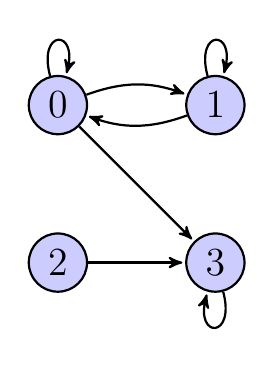
\begin{tikzpicture}[->,>=stealth',shorten >=1pt,auto,node distance=2cm,
 			thick,main node/.style={circle,fill=blue!20,draw,
 				font=\sffamily\Large\bfseries,minimum size=5mm}]
 			
 			\node[main node] (A) {$0$};
 			\node[main node] (B) [right of=A] {$1$};
 			\node[main node] (C) [below of=A] {$2$};
 			\node[main node] (D) [below of=B] {$3$};
 			
 			\path[every node/.style={font=\sffamily\small,
 				fill=white,inner sep=1pt}]
 			(A) edge [loop above] (A)
 			(A) edge [bend left=20] (B)
 			(A)edge (D)
 			(B) edge [loop above] (B)
 			(B) edge [bend left=20] (A)
 			(C) edge (D)
 			(D) edge [loop below] (D);
 		\end{tikzpicture}
 	\end{center}
 	
 	$R_1$ is not reflexive as every vertex doesn't include a loop (an arrow that goes from the vertex to the itself).\\
 	
 	Neither is it symmetric, as not all vertices is connected by arrows that goes to and from another arrow.\\ 
 	
 	It is transitive, as there are no simple paths connecting three vertices.\\
 	
 	$R_2$ has the following graph:
 	
 	\begin{center}
 		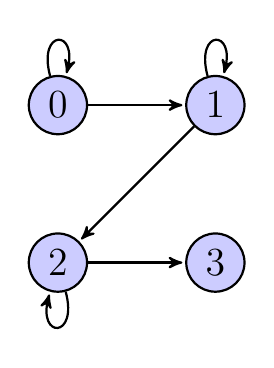
\begin{tikzpicture}[->,>=stealth',shorten >=1pt,auto,node distance=2cm,
 			thick,main node/.style={circle,fill=blue!20,draw,
 				font=\sffamily\Large\bfseries,minimum size=5mm}]
 			
 			\node[main node] (A) {$0$};
 			\node[main node] (B) [right of=A] {$1$};
 			\node[main node] (C) [below of=A] {$2$};
 			\node[main node] (D) [below of=B] {$3$};
 			
 			\path[every node/.style={font=\sffamily\small,
 				fill=white,inner sep=1pt}]
 			(A) edge [loop above] (A)
 			(A) edge (B)
 			(B) edge [loop above] (B)
 			(C) edge [loop below] (C)
 			(B) edge (C)
 			(C) edge (D);
 		\end{tikzpicture}
 	\end{center}
 	
 	This relation doesn't satisfy any properties as not all vertices have an edge loop, and all the vertices are connected in one direction only, and last there is a distinct path from $0$ through $1$ to $2$, but no path from $0$ to $2$.\\
 	
 	Let's look at the graph of $R_3$:
 	
 	\begin{center}
 		\begin{tikzpicture}[->,>=stealth',shorten >=1pt,auto,node distance=2cm,
 			thick,main node/.style={circle,fill=blue!20,draw,
 				font=\sffamily\Large\bfseries,minimum size=5mm}]
 			
 			\node[main node] (B) [left of=C] {$1$};
 			\node[main node] (C) [right of=B] {$2$};
 			
 			\path[every node/.style={font=\sffamily\small,
 				fill=white,inner sep=1pt}]
 			(B) edge [bend left=20] (C)
 			(C) edge [bend left=20] (B);
 		\end{tikzpicture}
 	\end{center}
 	
 	This relation however seems to satisfy the reflexive property as every vertex has an edge loop. Furthermore it must also be symmetric as every vertex is connected to another vertex by two arrows going out and in. And last, it also seems to be an transitive relation.\\
 	
 	The graph of $R_4$:
 	
 	\begin{center}
 		\begin{tikzpicture}[->,>=stealth',shorten >=1pt,auto,node distance=2cm,
 			thick,main node/.style={circle,fill=blue!20,draw,
 				font=\sffamily\Large\bfseries,minimum size=5mm}]
 			
 			\node[main node] (A) [left of =B] {$1$};
 			\node[main node] (B) [right of =A] {$2$};
 			\node [main node] (C)  [below of=A] {$3$};
 			\path[every node/.style={font=\sffamily\small,
 				fill=white,inner sep=1pt}]
 			(A) edge [bend left=20] (B)
 			(B) edge [bend left=20] (A)
 			(A) edge [bend left=20] (C)
 			(C) edge [bend left=20] (A);
 			
 		\end{tikzpicture}
 	\end{center}
 	
 	$R_4$ is not reflexive as no vertex contains an edge loop. That is:
 	
 	\cent{$\forall x,y \In A \exists(x,y) \In \doubleR^2  : (x,y)  \In R_4 \to x \neq y$}
 	
 	That says: \textit{"For all elements $x$ and $y$ of $A$, there exists a pair of reals of $x$ and $y$ such that, if it is an element of $R_4$, then $x$ and $y$ are not equal }.\\
 	
 	$R_4$ is symmetric as:
 	
 	\cent{$ \forall x,y \In A  \exists (x,y) \In \doubleR^2 : (x,y) \In R_4 \to (y,x) \In R_4  $}
 	
 	That says: For all elements $x$ and $y$ of $A$, there exists a pair of reals such that, if a pair of  $x$ and $y$ is an element of $R_4$, then a pair of $y$ and $x$ is also an element of $R_4$.\\
 	
 	$R_4$ is transitive as there are no elements of $R$ such that, whenever there are an element $(x,y)$, there is also an element  $(y,z)$.
 	The graph of $R_5$:
 	
 	\begin{center}
 		\begin{tikzpicture}[->,>=stealth',shorten >=1pt,auto,node distance=2cm,
 			thick,main node/.style={circle,fill=blue!20,draw,
 				font=\sffamily\Large\bfseries,minimum size=5mm}]
 			
 			\node[main node] (A) [left of =B] {$0$};
 			\node[main node] (B) [right of =A] {$1$};
 			\node [main node] (C)  [below of=A] {$2$};
 			\path[every node/.style={font=\sffamily\small,
 				fill=white,inner sep=1pt}]
 			(A) edge [loop above] (A)
 			(A) edge (B)
 			(A) edge (C)
 			(B) edge (C);
 		\end{tikzpicture}
 	\end{center}
 
 	$R_5$ is neither reflexive or symmetric as only one vertex contains an edge loop, and while all vertices might be connected, they are not connected bidirectional. But $R_5$ is transitive as there is elements of $R$ such that, whenever there is a mapping from $x$ to $y$, and $y \to z$, there is also a mapping from $x$ to $z$.\\
 	
 	The graph of $R_6$:
 	
 	\begin{center}
 		\begin{tikzpicture}[->,>=stealth',shorten >=1pt,auto,node distance=2cm,
 			thick,main node/.style={circle,fill=blue!20,draw,
 				font=\sffamily\Large\bfseries,minimum size=5mm}]
 			
 			\node[main node] (A) [left of =B] {$0$};
 			\node[main node] (B) [right of =A] {$1$};
 			\node [main node] (C)  [below of=A] {$2$};
 			\path[every node/.style={font=\sffamily\small,
 				fill=white,inner sep=1pt}]
 			(A) edge (B)
 			(A) edge (C);
 		\end{tikzpicture}
 	\end{center}
 
 	$R_6$ has no properties as none of them are satisfied. We'll make it short for now.
 	
 	The graph of $R_7$:
 	
 	\begin{center}
 		\begin{tikzpicture}[->,>=stealth',shorten >=1pt,auto,node distance=2cm,
 			thick,main node/.style={circle,fill=blue!20,draw,
 				font=\sffamily\Large\bfseries,minimum size=5mm}]
 			
 			\node[main node] (A) [above left of =C] {$0$};
 			\node[main node] (B) [above right of =C] {$2$};
 			\node [main node] (C)  [below left of=B] {$3$};
 			\path[every node/.style={font=\sffamily\small,
 				fill=white,inner sep=1pt}]
 			(A) edge (C)
 			(B) edge (C);
 		\end{tikzpicture}
 	\end{center}
 	
 	Again, no properties satisfied.\\
 	
 	Let's take a look on the last relation $R_8$:
 	
 	\begin{center}
 		\begin{tikzpicture}[->,>=stealth',shorten >=1pt,auto,node distance=2cm,
 			thick,main node/.style={circle,fill=blue!20,draw,
 				font=\sffamily\Large\bfseries,minimum size=5mm}]
 			
 			\node[main node] (A) [left of =B] {$0$};
 			\node[main node] (B) [right of =A] {$1$};
 			\path[every node/.style={font=\sffamily\small,
 				fill=white,inner sep=1pt}]
 			(A) edge [loop above] (A)
 			(B) edge [loop above] (B);
 		\end{tikzpicture}
 	\end{center}
 
 	$R_8$ is reflexive as all vertices have looops, but transitive, but not symmetric, as no edges is present. 
 
 	\Exercise{8.2.9}
 
	 \assignmentDescription
	 Let $R$ be a relation on $\doubleR$ such that $(x,y) \In R \leftrightarrow x \geq y $. Determine if $R$ satisfy any properties and justify your answer.\\
	  
	 \solution
	 $R$ must satisfy the property of reflexivity, as $R$ contain pairs $(x,x)$ for any element $x$ of $\doubleR$, since $x \geq x$.\\
	 
	 $R$ is not symmetric, as we for a particular element $x,y$ of $R$, can't find its inverse, as it would violate the size constraints on $R$.\\
	 
	 $R$ is transitive, as $R$ satisfies for $x \geq y \geq z$ the property of transitivity:
	 
	 \cent{$\forall x,y,z \In R : (x,y) \In R  \wedge (y,z) \In R \to (x,z) \In R$}
	 
	 \Exercise{8.2.14}
	 
	 \assignmentDescription
	 Let $O\In (x,y) \In \doubleZ^2$ such that $x-y = 2k-1$. Determine if $O$ satisfy any properties and justify your answer.\\
	 
	 \solution
	 First of all, every integer $x$ subtracted by $x$ is 0, and by definition of integer is even. Hence $O$ is not reflexive.\\
	 
	 By definition of symmetri, we demands that for every occurence of a pair $(a,b)$, there is also an inverted pair such that $(b,c)$.\\ 
	 
	 With regard to the constraints on $O$, we must require that every occurence of $(x,y)$ that complies with the constraints on $O$, there must also be an occurence of $(y,x)$ that also complies with the constraints on $O$.\\
	 
	 Let $k_1$ be the difference of two particular but arbitrary integers on the form $2q_i + c$ and $K_2$ the inverse difference:
	 
	 \cent{$k_1 = (2q_1+1) - 2q_2 = 2(q_1 - q_2) + 1, \quad q_1,q_2 \In \doubleZ$}
	 
	 \cent{$k_2 = 2q_2  - (2q_1 + 1) = 2(q_2 -q_1) - 1, \quad q_1,q_2 \In \doubleZ$}
	 
	 We observe that both $K_1$ and $K_2$ is on the form $2k +1$, which means that they are both odd. Hence they comply with the constraints on $O$, and as such, $O$ is symmetric.\\
	 
	 By definition of transitivity, we must require, that for every occurence of $(x,y)$ and $(y,z)$, there must also exists an occurence of $(x,z)$.\\
	 
	 We can visualize this in terms of $2q_i + c$ and the constraints set on $O$:
	 
	 \cent{$(2q_1+1,2q_2) \wedge (2q_3,2q_4 + 1) \to (2q_1 + 1, 2q_4+1)$}
	 
	 But as $(2q_1 + 1) - (2q_4 + 1) = 2(q_1 - q_2)$ is even, it violates the constraints set on $O$.\\ 
	 
	 Hence there do exists a series of elements such that $(x,y) \In O \wedge (y,z) \In O \to (x,z) \notin O$, and as such, $O$ is not transitive.
	 
	 \Exercise{8.2.21}
	 
 	\assignmentDescription
 	Let $X=\{a,b,c\}$ and $\script{P}(X)$ the powerset of $X$. Let $L$ be a relation on $\script{P(X)}$ such that, $|A| < |B|$ for every set $A \In \script{P}(x)$ and $B \In \script{P}(x) $.\\

	\solution
	We have the powerset of $X$ defined as:
	
	\cent{$\script{P}(x) = \{\{\emptyset\},\{a,b\},\{a,c\},\{b,c\},\{a\},\{b\},\{c\},\{a,b,c\}\}$}
	
	As the relation $L$ is the relation on $\script{P}(x)$ such that, $|A| < |B|$ for any $A \In \script{P}(x)$ and $B \In \script{P}(x)$. For a relation $R$ to be reflexive, it must contain elements such that, $(x,x) \In L$ for all elements of $X$. But that will imply a violation of the constraints set on $L$.\\
	
	Hence $L$ is not reflexive.\\
	
	As with regard to the constraints on $L$, there can't be an element of $L$ such that $|A| \geq |B| $.\\
	
	Hence $L$ is not symmetric.\\
	
	
	We know that $|X|=3$, and the element of the least cardinality in $\script{P}(X)$ must be $ 1 $ (we excludes the $\emptyset$, but if we imagine any mapping including the emptyset, it wouldn't change anything.) and the element of the greatest cardinal is $3$. Then we can for all elements $a  \In \script{P}(x)$, where $|a| = 1$, always assume a mapping of an element of cardinality of $1$, to an element of cardinality $ 2 $. And as of this, there must also exist an element with cardinality of $1$, to an element of cardinality of $3$.\\
	
	Hence $L$ is transitive.
	
	\Exercise{8.2.[34-36]}
	
	\assignmentDescription
	Let $R$ be some arbitrary relation on some set $A$. Show $R^{-1}$ maintains all properties of $R$.\\
	
	\solution
	Let $R : A \mapsto A^2$ be a relation on $A$, then we can show, that $R^{-1}$ maintains all the properties of its inverse. Consider the following statement:
	
	\cent{$\forall x,y \In A : (x,y) \In R \to (y,x) \In R^{-1}$}
	
	Which says, that if  $(x,y)$ is an element of $R$, then its inverse must by definition of an "\textit{inverse mapping}" be an element of $R^{-1}$, such that $(y,x) \In R^{-1}$.\\
	
	Let's assume $R$ is reflexive, then we can pick all elements that complies with the property of reflexivity:
	
	\cent{$\forall x \In A : x \In A \to (x,x) \In R$}
	
	The inverse of such an element maintains invariance with regard to order, which implies that the inverse of any relation maintains invariance with regard to reflexivity.\\
	
	Then let's assume $R$ is symmetric such that, for every element $ (x,y) $ of $R$  there is an inverse variant $ (y,x) $ of $R$. These elements still maintains invariance with regard to their properties, as they are each others inverse.\\ 
	
	Hence $R^{-1}$ maintains invariance with regard to symmetri.\\
	
	Finally, let's assume $R$ is transitive. We know by definition of transitivity, that whenever there is an element $(x,y)$ and $ (y,z) $ of $R$, then there must also be an element of $(x,z)$ of $R$.\\
	
	That means, we assume that there exists elements such that:
	
	\cent{$ (x,y) \In R \wedge (y,z) \In R \to (x,z)\In R$}
	
	Then we can safely assert, that similiar elements of  $R^{-1}$ exists such that:
	
	\cent{$ (z,y) \In R^{-1} \wedge (y,x) \In R^{-1} \to (z,x)\In R^{-1}$}
	
	Hence $R^-1$ maintains invariance with regard to transitivity.
	
	\Exercise{8.2.[37-42]}
	
	\assignmentDescription
	Let $A$ be some arbitrary set, and $R$ and $S$ relations on $A$. Determine if intersection or union maintains properties with regard to reflexivity, symmetry, and transitivity.\\
	
	\solution
	Let's consider $R$ and $S$ with regard to intersection and reflexitivity. We assume that $R$ and $S$ are reflexive, and as such, they must in fact contain the same element to satisfy the following property:
	
	\cent{$\forall x \In U : x \in A \to (x,x) \In R $}
	
	So the intersection of $R$ and $S$ must at least contain all the elements that satisfy the above criteria such that:
	
	\cent{$\forall (a,b) \In U : (x,x) \In R \to (x,x) \In S $}
	
	And as such, $R \cap S$ maintains invariance with regard to the property reflexitivity.\\
	
	What about the union and reflexivity?\\
	
	If $R$ and $S$ are both relations on $A$, and we assume they are reflexive, then they must again at least comprise the same elements that satisfy the property of reflexivity. That must imply that union also maintains invariance with regard to reflexivity.\\
	
	Let's assume that $R$ and $S$ is both symmetric, then we can consider $R \cap S$.  But we will also assume $R$ and $S$ to be disjoint sets, and therefore $R \cap S = \emptyset$.\\
	
	Hence $R \cap S$ is not guaranteed to maintain invariance with regard to symmetri.\\
	
	What about symmetry and union?\\
	
	Let's assume the same properties for $A$ and $B$ as before. That is, they are symmetric and disjoint. That means whenever $A$ and $B$ contains an element $(x,y)$, they also contains an element $(y,x)$. As of this, the union must comprise elements such that $(x,y) \In A \cup B \to (y,x) \In A \cup B$.\\ 
	
	Hence union maintains invariance with regard to symmetry.\\
	
	If we assume $A$ and $B$ to be transitive, what about $A \cap B$?\\
	
	By definition of transitivity, we can formulate in terms of an hypothesis and conclision. Let's consider the formal definition:
	
	\cent{$(x,y) \In R \wedge (y,z) \to (x,z)$}
	
	Which is a formula on the form $\phi \wedge \psi \to \gamma$. The formula is only false for $\phi = true$ and $\psi = false$ which is hypothesis and conclusion, respectively.\\
	
	So, a relation is not transitive for the case where the hypothesis is true and conclusion is false. As we assume $A$ and $B$ to be transitive, the intersection of $A$ and $B$ must either contain the hypotesis and conclusion, or parts of the hypothesis or the conclusion, which isn't enough to qualify for intransitivity.\\
	
	Hence intersection maintains invariance with regard to transitivity.\\
	
	Then let's consider the union of $A$ and $B$ and assume they complement each other with regard to the hypothesis. That is, the relation $R$ contains an element $(x,y)$ and $S$ contains an element $(y,z)$, but none of them contains an element $(x,z)$. Then $R \cup S$ is not transitive as it contains the elements $(x,y)$ and $(y,z)$, but not the element $(x,z)$. That makes the hypothesis true and conclusion false.\\
	
	Hence union is not guaranteed to maintain invariance with regard to transitivity.
	
	\Exercise{8.3.1}
	
	\assignmentDescription
	Let $A=\{a,b,c,d,e\}$ and $R$ a relation on $S$. Consider the following relations:
	
	\mAlign{&_cR_b \quad  _cR_c \quad _aR_c \quad  _bR_c \\
					&_aR_d \quad  _cR_a \quad _e R_d  \quad _cR_a } 
	
	Determine for any statement if one of the above is an element of $R$.\\
	
	\solution
	
	\begin{enumerate}[label=\defaultEnumerateLabel]
		\item R is reflexive\\
		
		If $R$ is reflexive, then $_cR_c$ must be true.
		
		\item R is symmetric
		
		If $R$ is symmetric, then $_aR_c$ and $_cR_a$ must be true.
		
		\item If R is transitive
		
		If $R$ is transitive, then $_cR_c$, $_cR_a$, and $_cR_a$ must be true.
		
		\item If $R$ is an equivalence relation
		
		If $R$ is an equivalence relation, then $_cR_c$, $_aR_c$, $_cR_a$, $_cR_c$, $_cR_a$, and $_cR_a$ must be true.
	\end{enumerate}
	\Exercise{8.3.2}
	
	\assignmentDescription
	Let $A=\{0,1,2,3,4\}$ and $R$ be a relation on $A$. For each given partitions of $A$, find the ordered pairs of $R$.\\
	
	\solution
	
	\begin{enumerate}[label=\defaultEnumerateLabel]
		\item $\{0,2\}$, $\{1\}$, $\{3,4\}$
		
		Let's define equivalence relations $S_i$ on each subset of $A$:
		
		\mAlign{S_1&= \{(0,0),(2,2),(0,2),(2,0)\} \\ S_2 &= \{(1,1)\} \\ S_3 &= \{(3,3),(4,4),(3,4),(4,3)\} \\}
		
		Then $R = S_1 \cup S_2 \cup S_3$.
		
		
		\item $\{0\}$, $ \{1,3,4\} $, $ \{2\} $
		
		Again, we define all the equivalence relations on each given subset:
		
		\mAlign{S_1&= \{(0,0)\} \\ S_2 &= \{(1,1),(3,3),(4,4),(1,3),(1,4),(3,1),(4,1),(3,4),(4,3)\} \\ S_3 &= \{(2,2)\} \\}
		
		And as before, $R = S_1 \cup S_2 \cup S_3$.
		
		
		\item $\{0\},\{1,2,3,4\}$
		
		\mAlign{S_1&= \{(0,0)\} \\ S_2 &= R \setminus S_1 \\}
		
		And $R = S_1 \cup S_2$,
	\end{enumerate}
	
	\Exercise{8.3.4}
	
	\assignmentDescription
	Let $A=\{a,b,c,d\}$ and $R=\{(a,a),(b,b), (b,d),(c,c),(d,b),(d,d)\}$ be an equivalence relation on $A$. Determine the equivalence classes of $R$.\\
	
	\solution
	
	We can define all the equivalence classes as:
	
	\mAlign{[a] &= \{x \in R | (x,y) \In R\} = \{a\} \\
					[b] &= \{x \in R | (x,y) \In R\} = \{b,d\} \\
					[c] &= \{x \in R | (x,y) \In R\} = \{c\} \\
					[d] &= \{x \in R | (x,y) \In R\} = \{b,d\}}
	
	\Exercise{8.3.9}
	
	\assignmentDescription
	Let $X=\{-1,0,1\}$ and $A=\script{X}$ such that:
	
	\cent{$A  = \{\{\emptyset\},\{-1\},\{0\},\{1\},\{-1,0\},\{-1,1\},\{0,1\},\{-1,0,1\}\}$}
	
	\solution
	
	\mAlign{[\{-1\}] &= \{x \in R | (x,y) \In R\} = \{\{-1\},\{-1,0\}\} \\
		[\{0\}] &= \{x \in R | (x,y) \In R\} = \{\{0\},\{-1,0,1\},\{-1,1\}\} \\
		[\{1\}] &= \{x \in R | (x,y) \In R\} = \{\{1\},\{0,1\}\} \\
		[\{-1,0\}] &= \{x \in R | (x,y) \In R\} = \{\{-1\},\{-1,0\}\} \\
		[\{-1,1\}] &= \{x \in R | (x,y) \In R\} = \{\{0\},\{-1,0,1\},\{-1,1\}\} \\
		[\{-1,0,1\}] &= \{x \in R | (x,y) \In R\} = \{\{0\},\{-1,0,1\},\{-1,1\}\}}
	
	\Exercise{8.3.13}
	
	\assignmentDescription
	Let $A$ be the set of strings such that the length of every string is 4 and comprise a's and b's. Then let $R$ be a relation on $A$ such that, it relates every element of $A$ if, and only if, they begins with the same two letters.\\
	
	\solution
	\mAlign{
		[\{AAAA\}] &= \{x \in R | (x,y) \In R\} = \{\{AAAA\},\{AABA\},\{AABB\},\{AAAB\}\} \\
		[\{AABA\}] &= \{x \in R | (x,y) \In R\} = \{\{AAAA\},\{AABA\},\{AABB\},\{AAAB\}\} \\
		[\{AAAB\}] &= \{x \in R | (x,y) \In R\} = \{\{AAAA\},\{AABA\},\{AABB\},\{AAAB\}\} \\
		[\{AABB\}] &= \{x \in R | (x,y) \In R\} = \{\{AAAA\},\{AABA\},\{AABB\},\{AAAB\}\} \\
		[\{ABBA\}] &= \{x \in R | (x,y) \In R\} = \{\{ABBA\},\{ABBB\},\{ABAB\,\{ABAA\}\} \\
		[\{ABBB\}] &= \{x \in R | (x,y) \In R\} = \{\{ABBA\},\{ABBB\},\{ABAB\,\{ABAA\}\} \\
		[\{ABAB\}] &= \{x \in R | (x,y) \In R\} = \{\{ABBA\},\{ABBB\},\{ABAB\,\{ABAA\}\} \\
		[\{ABAA\}] &= \{x \in R | (x,y) \In R\} = \{\{ABBA\},\{ABBB\},\{ABAB\,\{ABAA\}\} \\
		[\{BAAA\}] &= \{x \in R | (x,y) \In R\} = \{\{BAAA\},\{BAAB\},\{BABA\},\{BABB\}\} \\
		[\{BAAB\}] &= \{x \in R | (x,y) \In R\} = \{\{BAAA\},\{BAAB\},\{BABA\},\{BABB\}\} \\
		[\{BABA\}] &= \{x \in R | (x,y) \In R\} = \{\{BAAA\},\{BAAB\},\{BABA\},\{BABB\}\} \\
		[\{BABB\}] &= \{x \in R | (x,y) \In R\} = \{\{BAAA\},\{BAAB\},\{BABA\},\{BABB\}\} \\
		[\{BBAA\}] &= \{x \in R | (x,y) \In R\} = \{\{BBAA\},\{BBAB\},\{BBBB\},\{BBAB\}\} \\
		[\{BBAB\}] &= \{x \in R | (x,y) \In R\} = \{\{BBAA\},\{BBAB\},\{BBBB\},\{BBAB\}\} \\
		[\{BBBB\}] &= \{x \in R | (x,y) \In R\} = \{\{BBAA\},\{BBAB\},\{BBBB\},\{BBAB\}\} \\
		[\{BBAB\}] &= \{x \in R | (x,y) \In R\} = \{\{BBAA\},\{BBAB\},\{BBBB\},\{BBAB\}\}}
	
	\Exercise{8.3.19}
	\assignmentDescription
	Let $A$ be all the students at a college. Each student is either major or double major. Let $R$ be a relation on $A$ such that, $R$ relates elements of $A$ that has the same major. Prove that $R$ is an equivalence relation.\\
	
	\solution
	First of all, let's partition $A$ into two partitions $X$ and $Y$ such that, $X$ is the set of all elements of $A$ that have a major, and $Y$ is the set of all elements of $A$ that has a double major. If we construct relations on $X$ and $Y$ such that, they all satisfy the three properties that is required for relations to be equivalence relations, then the union of them must be $R$. Hence $R$ must be an equivalence relation on $A$, \\
	
	First we have to construct relations $X_r$ and $Y_r$ on $X$ and $Y$ in accordance with the above:\\
	
	 We can construct relations $X_r$ and $Y_r$ such that $\forall x \In X : (x,x) \In  X_r  $ and $\forall x \In Y : (y,y) \In  Y_r  $. That means, for every element $x$ of $X$ and $y$ of $Y$, we construct elements such that $(x,x) \In X_r$ and $(y,y) \In Y_r$. Hence $X_r$ and $Y_r$ are reflexive relations on $X$ and $Y$, respectively.\\
	 
	 We can then expand our relations so that $\forall x,y \In X: (x,y) \In X_r \to (y,x) \In X_r$ and $\forall y,z \In Y_r : (y,z) \to (z,y) \In Y_r$. That means, for every occurence of $(x,y) $ in $X_r$, there must also exists an element $(y,x)$ in $X_r$, and the same applies for $Y_r$. That implies, by definition of symmetri, that $X_r$ and $Y_r$ must be symmetric relations on $X$ and $Y$, respectively.\\
	 
	 Last, we must construct $X_r$ and $Y_r$ such that they are transitive. By definition of transitivity, whenever there exists a relation from an element $x$ to some element $y$, and a relation from that $y$ to some element $z$, there must also exists a relation from $x$ to $z$. That means, we must require from $X_r$ that $\forall x,y,z \In X : (x,y) \In X_r \wedge (y,z) \In X_r \to (x,z) \In X_r$. And this of course also applies for $Y_r$. Hence $X_r$ and $Y_r$ are transitive relations on $X$ and $Y$, again with regard to $X$ and $Y$. \\
	 
	 This leads us to the grand finale, as we remember that $X$ and $Y$ are partitions of $A$, and as such, $X_r$ and $Y_r$ must also be partitions of $R$. Since we constructed $X_r$ and $Y_r$ according to our requirements, that means they are both reflexive, symmetric, and transitive; they are equivalence relations on their respective partitions.  The union of $X$ and $Y$ must by definition of union be the set $A$, and the union of $X_r$ and $Y_r$ must also be the relation $R$.\\
	 
	 Hence $R$ is an equivalence relation on $X$.\\
	 \QED
	
	\Exercise{8.3.34}
	
	\Prove
	Prove the following relation to be an equivalence relation:
	
	\cent{$(p,q) \In R \leftrightarrow \sqrt{p^2 + q^2} \leq c, \quad (p,q) \In \doubleR^2, c \In \doubleR^+$}
	
	Where $c$ is some small positive number.\\
	
	\solution
	
	\begin{itemize}
		\item Reflexive
		
		The distance between any given points $p$ and $q$, we assume identical, must be less or equal some small positive number $c$. In fact, the distance must exactly be 0. Since $c > 0$, a pair of these points meets the criterias set for $R$. Hence any relation $R$ considered reflexive must comprise pairs that satisfy this condition.\\
		
		We can actually verify this, by determine $|pp|$:
		
		\cent{$ |pp| = \sqrt{(x - x)^2 + (y - y)^2} = 0 $}
		
		\item Symmetric
		
		For any given points $p$ and $q$, not identical, that satisfies $|p-q| \leq c$, also satisfies $|q-p| \leq c$. Hence any relation considered symmetric must comprise pairs that satisfy this condition.\\
		
		Again, we can verify by insertion:
		
		\cent{$\sqrt{(x_2 - x_1)^2 + (y_2 - y_1)^2}$}
		
		\item Transitive
		
		For any given points $p$ and $q$, where $|q-p| \leq k$, for $k < c$, there must exists a point $r$, such that $|r-q| \leq c - k$. Then it follows that $|r-q| \leq c$. Any relation that are considered transitive must comprise pairs which satisfies this condition.\\
	\end{itemize}
	
	Since all the properties can be satisfied, any relation $R$ that comprise pairs such that, the distance between its points never exceeds some small positive number $c$, can be considered an equivalence relation.\\
	\QED
	
	\Exercise{8.3.[36-41]}
	
	\assignmentDescription
	Let $A$ be some set and $R$ its equivalence relation.\\
	
	Prove any given statement without the use of lemmas or theorems.\\
	
	\solution
	\begin{itemize}
		\item $\forall x : x \In A \to x \In [x]$
		
		This is true as a result of $R$ being reflexive. That is, $\forall x : x \In A \to (x,x) \In R$. As such, the equivalence relation $R$ must at least comprise pairs of $x$. Hence $x$ is an element of the equivalence class of $x$.
		
		\item $\forall x,y \In A : y \In [x] \to (x,y) \In R$
		
		Yes, it follows from the fact, that $R$ satisfies the property of symmetry. This means, we can rewrite the statement by definition of symmetry. That is, $R$ relates $x$ and $y$. We can substitute $(y,x)\In R$ for $y \In [x]$ in the given statement:
		
		\cent{$\forall x,y \In A : (y,x) \In R \to (x,y) \In R$}
		
		Which is the definition of symmetri. This means, with regard to the properties of $R$, we can conclude that the formula holds.
		
		\item $\forall x,y,z \In A : (y,z) \In R \wedge z \In [x] \to y \In [x]$
		
		Let's rewrite the statement by substituting $(z,x)\In R$ for $z \In [x]$, and $(y,x \In R)$ for $y \In [x]$ :
		
		\cent{$\forall x,y,z \In A : (y,z) \In R \wedge (z,x)\In R \to (y,x) \In R$}
		
		We can do that because, if any element $a$ is part of some equivalence class of some other element $b$, they must be related by some relation $R$. This happens to be our equivalence relation $R$, which is an equivalence class and as such, satisfies the property of transitivity. We note that the rewritten statement is indeed the definition of transitivity.
		
		\item $\forall x,y : [x] = [y] \to (x,y)\In R$
	\end{itemize}
		
	We know, by definition of equivalence classes, that any element $b$ of some equivalence class $[a]$, is related to $a$ by some relation $R$. If that's not the case, then they are not related at all.\\ 
	
	In our context, $R$ is an equivalence relation on $A$. All properties that makes $R$ an equivalence relation can be satisfied even if $R$ only relates each element to itself. That implies, that any particular, but arbitrarily chosen, equivalence class $[a]$ is disjoint from any other particular, but arbitrarily chosen, equivalence class $[b]$. Hence $a$ and $b$ are not related by $R$.\\
	
	But if $R$ actually relates some element $a \In A$ to some element $b \In A$, then $R$ must also relate $b$ to $a$, due to symmetry. And if $a$ and $b$ are not related by $R$ to any other elements of $A$, then the equivalence class of $a$ and $b$ only comprise elements of itself and the element related to by $R$. Hence $R$ relates $a$ and $b$.\\
	
	Then we can extend our assumption from the previous step, that $R$ does in fact relate $b$ to some other particular, but arbitrarily chosen, element $c$. Then $R$ must also relate $a$ to $c$ due to transitivity. Again, the equivalence class of $a$ and $b$ only comprise elements of itself and the elements they are related to by $R$. In our case, that would be $a,b,c$ for each. Hence $R$ relates $a$ and $b$.\\
	\QED
	
	\Exercise{8.5.3}
	\assignmentDescription
	Let $S$ be the set of all strings of $a$'s and $b$'s. Define a relation $ R $ on $ S $ such that:
	
	\cent{$ R = \{s,t \In S | (s,t) \In S^2 \to L(s) \leq L(t)\}$} 
	
	Where $L(x)$ denotes the length of any string $x$.\\
	
	\solution
	
	For all elements $(s,t) \In R$, $R$ is antisymmetric if the following is valid:
	
	\cent{$\forall s,t \In S : (s,t) \In R \wedge (t,s) \In R \to (s = t)$}
	
	As $R$ relates elements $s,t \In S$ such that, the length of $s$ is less or equal than the length $t$, we can rewrite the above to:
	
	\cent{$\forall s,t \In S : ((L(s) \leq L(t)) \wedge (L(s) \geq L(t))\to (s = t)$}
	
	By using logic, we can again rewrite in terms of a particular element $(x,y)$: 
	
	\cent{$(L(x) \leq L(y)) \wedge (L(x) \geq L(y))\to (x = y)$}
	
	The goal is to determine a false interpretation. Let's evaluate for a particular pair $(x,y)$, where the length of $x$ is greater than the length of $y$. Then the conclusion is false, and for the hypothesis to be true, both elements need to be greater and less than the other (refering to the length of these). Which of course is impossible. We can in fact rewrite the formula as a consequence of our choice:
	
	\cent{$(L(x) < L(y)) \wedge (L(x) > L(y))\to \neg(x \neq y)$}
	
	As we notice, the above formula is on the form:
	
	\cent{$ \phi \wedge \neg \phi\to \psi$}
	
	Which is what we call a  \textit{tautology}, a formula that is true for all its interpretations. Hence $R$ is indeed antisymmetric.\\
	\QED
	
	\Exercise{8.5.5}
	\assignmentDescription
	Let $R$ be a relation on $\doubleR^2$ such that:
	
	\cent{$R = \{ a,b,c,d \In \doubleR | (a < c) \vee ((a = c) \wedge (b \leq d))\}$}
	
	Is $R$ a partial order relation?\\
	
	\solution
	For $R$ to be a partial order, it must be reflexive, asymmetric, and transitive. Let's proceed by proving each property.\\
	
	For any particular distinct pair of a pair of reals $((x,x),(x,x))$, we can show that $R$ is reflexive. Let's insert in the definition of $R$ and evaluate:
	
	\cent{$(x < x) \vee ((x = x) \wedge (x \leq x))$}
	
	As the above is true for this particular interpretation, it is true for every interpretations of this kind. Hence $R$ is reflexive.\\
	
	Then we can try to determine if $R$ is antisymmetric. We can first try to consider all elements such that, $a=c$ and $b = d$. That is, we want to know if any two pairs of  $((a,b),(a,b))$ exists. We can safely assert this, as we have already set $a=c$ and $b=d$. And this is commutative operations, so at least $R$ is asymmetric. But we can as well easily conclude that $R$ can't be symmetric, by consider all elements where $b < d$ or $a< c$. As these operations are not commutative in the sense, that $a$ can't be greater and less than any other element at the same time. Hence $R$ is antisymmetric.\\
	
	Last and finally, we need to show, that $R$ is transitive. Let's again focus on a particular element $((a,b),(c,d)) \In R$, where either $a < c$ or $a = c$ and $b \leq d$. We know, by definition of transitive, that whenever there exists an element $(a,b)$ and $(b,c)$, there must also exists an element $(a,c)$. Then we can assume the existence of another particular element $((c,d),(e,f)) \In R$, where either $c < e$  or $c=e$ and $d \leq f$. Then the definition of transitivity says, that there must also exists an element $((a,b),(e,f)) \In R$, where either $a<e$ or $a=e$ and $b \leq f$. We can in fact assert its truthfulness by considering the following statement:
	
	\cent{$(a < c < e) \vee (a = c = e) \wedge (b \leq d \leq f)$}
	
	Here we see, that whenever their exist two elements $((a,b),(c,d)) \In R$ and $((c,d),(e,f)) \In R$, which elements satisfies the above, we can always find an element such that$((a,b),(e,f)) \In R$. Hence $R$ is transitive.\\
	
	$R$ is reflexive, asymmetric, and transitive. Hence $R$ is a partial ordered relation.\\
	\QED
	
	\Exercise{8.5.6}
	
	\assignmentDescription
	Let $P$ be all human beings ever lived on earth, and let $R$ be a relation on $P$. We define $R$ as:
	
	\cent{$R = \{s,r \In P | (r < s) \vee (r = s)\}$}
	
	Where $<$ denotes an \textit{ancestor of} relation.\\
	
	Prove or give a counter example that $R$ is a partial ordered relation.\\
	
	\myRemark
	First some remarks about our notation. As we use the \textit{less than} operator to denote an \textit{ancestor of} relation, and an \textit{equal} operator to denote \textit{identical to} relation, we can rewrite the given statement in terms of an \textit{less or equal than} operator:
	
	\cent{$R = \{s,r \In P | (r \leq s)\}$}
	
	\solution
	Initially we must show, that $R$ is reflexive. As we know, that $R$ relates all elements that are identical, we know that $R$ is indeed reflexive. We can show that by inserting $ (x,x) $ in the definition of $R$:
	
	\cent{$x \leq x$}
	
	This must apply for all particular $x$. Hence $R$ is reflexive.\\
	
	Then we can show that $R$ is antisymmetric by process some important properties of the \textit{less than} operator. $\leq$ is not commutative in the sense, that $a$ might be less than $b$, but it can not be greater than $b$ at the same time. The only comparison operator that is commutative in this context, is the $=$ operator. With this in mind, we can evaluate a particular element $(x,y)$, where $x$ is an ancestor of $y$, but not the other way around. We can realize that when inserting in the definition of $R$:
	
	\cent{$ x \leq y \quad y \not \leq x $}
	
	hence $R$ is antisymmetric.\\
	
	$R$ must also be transitive due to the before mentioned property of $\leq$ operator. Let's assume $(x,y) \In R$, where $x$ is an ancestor of $y$. Then we can pick another particular pair $(y,z)\In R$, such that $y$ is ancestor of some element $z$. As $z$ is parent to $y$, it is grand parent to $x$, as $y$ is parent to $x$. Again, we can consider the definition of $R$:
	
	\cent{$x < y < z$}
	
	Hence $R$ is transitive.\\
	
	With all this in mind, we can conclude that $R$ is a partial ordered relation on $P$.\\
	\QED
	
	\Exercise{8.5.7}
	\assignmentDescription
	Let $R$ be a relation on $\doubleZ$ such that, it relates two elements $m$ and $n$, if, and only if, every primefactor of $m$ is a prime factor of $n$.
	
	\solution
	As every primefactorizations of some integer $m$ is unique, $R$ must relate identical elements.\\
	
	As of this, $R$ must be:
	\begin{itemize}
		\item Reflexive\\
		$R$ only relates identical elements, which is the definition of the property reflexive.
		\item Symmetric and antisymmetric\\
		It is both, as both definitions are satisfied.
		\item Transitive\\
		As the property of transitivity is satisfied.
	\end{itemize}
	Hence $R$ is a partial ordered relation.\\
	\QED
 
	\Exercise{8.5.10}
	
	\assignmentDescription
	Suppose $R$ and $S$ are antisymmetric relations on a set $A$. Must $R \cup S$ be antisymmetric due to the properties of $R$ and $S$?\\
	
	\solution
	
	No, not at all. Let $T = \{(1,2),(2,3),(3,2),(2,1)\}$ be an symmetric relation on $A = \{1,2,3\}$. Then we can partition $T$ into two sets $R = \{(1,2),(2,3)\}$ and $S = \{(3,2),(2,1)\}$. It is clear to us, that the union of $R$ and $S$ is $T$.\\
	
	Hence the given statement is false.\\
	\QED 
	
	\Exercise{8.5.14}
	
	\assignmentDescription
	Let $A=\{a,b,c\}$. Describe all partial partial order relations of $A$ for which $a$ is either maximal or minimal element.
	
	\solution
	Let's first develop the Hasse diagram for the full partial order relation:
	
	\begin{center}
		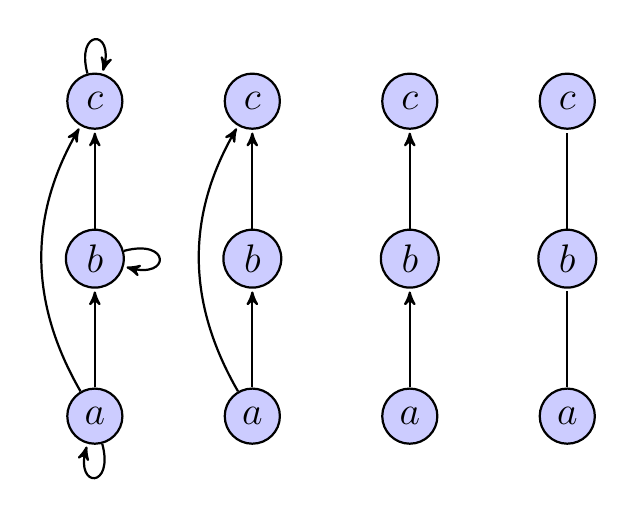
\begin{tikzpicture}[->,>=stealth',shorten >=1pt,auto,node distance=2cm,
			thick,main node/.style={circle,fill=blue!20,draw,
				font=\sffamily\Large\bfseries,minimum size=7mm}]
			
			\node[main node] (A) {$c$};
			\node[main node] (B) [below of=A] {$b$};
			\node[main node] (C) [below of=B] {$a$};
			
			\node[main node] (D) [right of=A]{$c$};
			\node[main node] (E) [below of=D] {$b$};
			\node[main node] (F) [below of=E] {$a$};
			
			
			\node[main node] (G) [right of=D]{$c$};
			\node[main node] (H) [below of=G] {$b$};
			\node[main node] (I) [below of=H] {$a$};
			% Hasse diagram
			\node[main node] (J) [right of=G]{$c$};
			\node[main node] (K) [below of=J] {$b$};
			\node[main node] (L) [below of=K] {$a$};
			
			\path[every node/.style={font=\sffamily\small,
				fill=white,inner sep=1pt}]
			(A) edge [loop above] (A)
			(B) edge (A)
			(B) edge [loop right] (B)
			(C) edge (B)
			(C) edge [loop below] (C)
			(C) edge [bend left] (A)
			
			(E) edge (D)
			(F) edge (E)
			(F) edge [bend left] (D)
			
			(H) edge (G)
			(I) edge (H)
			
			(K) [-] edge (J)
			(L)  edge (K);
		\end{tikzpicture}
	\end{center}

	As we can se from the figures above, the only partial ordered relation for which $a$ is the maximal element, must be $R = \{(a,a)\}$. Because $a$ will be the minimal element in any pair  of $a$ and every other element of $A$. As of this, $a$ will be minimal element of any remaining partial ordered relations on $R$ that exists.\\
	\QED
	
	\Exercise{8.5.20}
	
	\assignmentDescription
	Let $S=\{0,1\}$ and let $R\In S^3$ be a partial ordered relation such that:
	
	\cent{$((a,b,c),(d,e,f)) \In R \leftrightarrow a \leq d \wedge b \leq e \wedge c \leq f$}
	
	\solution
	23
	
	\begin{center}
		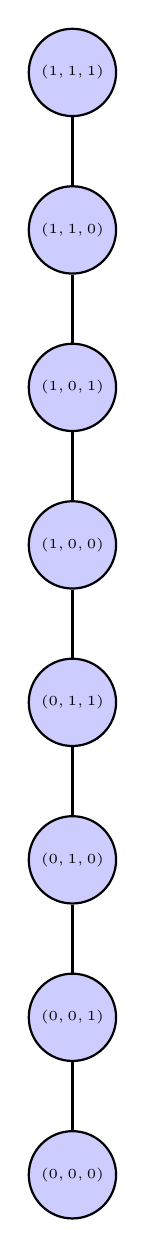
\begin{tikzpicture}[auto,node distance=2cm,
			thick,main node/.style={circle,fill=blue!20,draw,
				font=\sffamily\tiny\bfseries,minimum size=5mm}]
			
			\node[main node] (A) {$(1,1,1)$};
			\node[main node] (B) [below of=A] {$(1,1,0)$};
			\node[main node] (C) [below of=B] {$(1,0,1)$};
			\node[main node] (D) [below of=C] {$(1,0,0)$};
			\node[main node] (E) [below of=D] {$(0,1,1)$};
			\node[main node] (F) [below of=E] {$(0,1,0)$};
			\node[main node] (G) [below of=F] {$(0,0,1)$};
			\node[main node] (H) [below of=G] {$(0,0,0)$};
			
			\path[every node/.style={font=\sffamily\small,
				fill=white,inner sep=1pt}]
			(G) edge (H)
			(F) edge (G)
			(E) edge (F)
			(D) edge (E)
			(C) edge (D)
			(B) edge (C)
			(A) edge (B);
			
		\end{tikzpicture}
	\end{center}

		
	\Exercise{8.5.40}

	\section{Sums, graphs, tree, cardinality, and sequences}
	
	Exercises in this section will not undertake the same elaborate description as exercises in other sections.
	
	\Exercise{5.1.[1-4]}
	
	\assignmentDescription
	Evaluate any given sequences up to $k=4$
	
	\solution
	
	\begin{enumerate}
		\item $ a_j = \dfrac{k}{10+k}, \quad i \geq 1$
		
		\mAlign{
			a_1 &= \frac{1}{10+1} = \frac{1}{11} \\
			a_2 &= \frac{2}{10+2} = \frac{2}{12} = \dfrac{1}{6}\\
			a_3 &= \dfrac{3}{10+3} = \dfrac{3}{13} \\
			a_4 &= \dfrac{4}{10+4} = \dfrac{4}{14} = \dfrac{2}{7}
		}
		
		\item $ b_j = \dfrac{5-j}{5+j}, \quad j \geq 1$
		
		\mAlign{b_1 &= \dfrac{5-0}{5+0} = \dfrac{5}{5} = 1\\
					 b_2 &= \dfrac{5-1}{5+1} = \dfrac{4}{6} = \dfrac{2}{3} \\
				 	 b_3 &= \dfrac{5-2}{5+2} = \dfrac{3}{7} \\
			 	 	 b_4 &= \dfrac{5-3}{5+3} = \dfrac{2}{8} = \dfrac{1}{4}}
		
		\item $c_i = \dfrac{(-1)^i}{3^i}, \quad i \geq 0$
		
		\mAlign{c_0 &= \dfrac{(-1)^0}{3^0} = \dfrac{1}{1} = 1 \\
					 c_1 &= \dfrac{(-1)^1}{3^1} = - \dfrac{1}{3} \\
				 	 c_2 &= \dfrac{(-1)^2}{3^2} = \dfrac{1}{9} \\
			 	     c_3 &= \dfrac{(-1)^3}{3^3} = -\dfrac{1}{27}}
		
		\item $d_m = 1 + \parenthesis{\dfrac{1}{2}}^m = 1 + \dfrac{1}{2^m}, \quad m \geq 0$
		
		\mAlign{ d_0 &= 1 + \dfrac{1}{2^0} = 1 + \dfrac{1}{1} = 2 \\
					 d_1 &= 1+ \dfrac{1}{2^1} = 1+ \dfrac{1}{2} = \dfrac{2}{2} + \dfrac{1}{2} = \dfrac{2+1}{2} = \dfrac{3}{2} \\
				 	 d_2 &= 1 + \dfrac{1}{2^2} = 1 + \dfrac{1}{4} = \dfrac{4}{4} + \dfrac{1}{4} = \dfrac{4+1}{4} = \dfrac{5}{4} \\
			 		 d_3 &= 1 + \dfrac{1}{2^3} = 1+\dfrac{1}{8} = \dfrac{8}{8} + \dfrac{1}{8} = \dfrac{8+1}{8}=\dfrac{9}{8}}
		
	\end{enumerate}
	\Exercise{5.1.[19-22]}
	
	\assignmentDescription
	Evaluate any given sum
		
	\begin{enumerate}
		\item $\sum_{k=1}^{5} = (k+1)$
		
		\cent{$\sum_{k=1}^{5} = 2+3+4+5+6 = 21$}
		
		\item $\prod_{k=2}^{2} = k^2$
		
		\cent{$\prod_{k=2}^{2} = 4 \cdot 9 \cdot 16 = 36 \cdot 16 = 576$}
		
		\item $\sum_{k=1}^{3} = \parenthesis{k^2 + 1}$
		
		\cent{$\sum_{k=1}^{3} = 2 + 5 + 10 = 17$}
		
		\item $\prod_{j=0}^{4} = \prod_{j=1}^{4} = (-1)^j   $
		
		\cent{$\prod_{j=1}^{4} =  (-1) \cdot 1 \cdot  (-1) \cdot 1 = 1$}
		
	\end{enumerate}
	
	\Exercise{5.1.[43-45]}
	
	\assignmentDescription
	Write any given series in terms of summation or product notation
	
	\begin{enumerate}
		\item $1^2 - 2^2 + 3^2 - 4^2 + 5^2 - 6^2 + 7^2$
		
		\cent{$\sum_{i=0}^{6} (-1)^i (1+i)^2$}
		
		\item $(1^3-1)-(2^3-1)+(3^3-1)-(4^3 - 1) + (5^3 -1)$
		
		\cent{$\sum_{i=0}^{4} = (-1)^i \parenthesis{(1+i)^3 -1}$}
		
		\item $\parenthesis{2^2-1}\parenthesis{3^2 -1} \parenthesis{4^2 -1}$
		
		\cent{$\prod_{i=2}^{4} (i^2 -1)$}
		
	\end{enumerate}
	
	\Exercise{1.4.[8,9]}
	\solution
	\cent{$\text{inc}_1(v_1) = \{e_1,e_2,e_3\}, \quad inc_2(v_2) = \{e_1,e_2,e_7\}$}
	
	\cent{$\text{adj}_1(v_3) = \{v_1,v_2\}, \quad adj_2\{v_1,v_2\}$}
	
	\cent{$\text{adj}_1(e_1) = \{e_2,e_3,e_8,e_9\}, \quad \text{adj}_2(e_1) = \{e_2,e_7\}$}
	
	\cent{$\text{lps}_1 = \{(v_2,e_6),(v_3,e_7), \quad \text{lps}_2 = \{(v_1,e_1),(v_2,e_3)\}\}$}
	
	\cent{$\text{par}_1 = \{(e_4,e_5)\}, \quad \text{par}_2 = \{(e_4,e_5)\}$}
	
	\cent{$\text{iso}_1 =\{v_6\}, \quad \text{iso}_2 = \{v_4\}$}
	
	\cent{$deg_1(v_3) = 5, \quad deg_2(v_3) = 2$}
	
	\Exercise{4.9.1}
	
	\mAlign{V &= \{v_1,v_2,v_3,v_4,v_5,v_6\} \\
				 E &= \{e_1,e_2,e_3,e_4,e_5,e_6\}}
	
	\mAlign{\text{deg}(v_1) &= 3 \\
				\text{deg}(v_2) &= 2 \\
				\text{deg}(v_3) &= 4 \\
				\text{deg}(v_4) &= 2 \\
				\text{deg}(v_5) &= 1 \\
				\text{deg}(v_6) &= 0}
	
	\cent{$\sum \text{deg}(V) = 3 + 2 + 4 + 2 + 1 + 0 = 12$}
	
	\cent{$|E| = 6$}
	
	\Exercise{4.9.[5-8]}
	
	\begin{figure}[H]
		\centering
		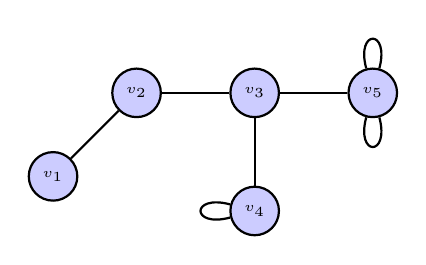
\begin{tikzpicture}[-,auto,node distance=1.5cm,
			thick,main node/.style={circle,fill=blue!20,draw,
				font=\sffamily\tiny\bfseries,minimum size=1mm}]
			
			\node[main node] (A) {$v_1$};
			\node[main node] (B) [above right of=A] {$v_2$};
			\node[main node] (C) [right of=B] {$v_3$};
			\node[main node] (D) [below of=C] {$v_4$};
			\node[main node] (E) [right of=C] {$v_5$};
			\tikzstyle{every loop}=[-]
			\path[-,every node/.style={font=\sffamily\small,
				fill=white,inner sep=1pt}]
			(A) edge (B)
			(B) edge (C)
			(D) edge (C)
			(C) edge (E)
			(D) [] edge [loop left](D)
			(E) [] edge [loop above](E)
			(E) [] edge [loop below](E);
			
			
		\end{tikzpicture}
		\caption{4.9.5}
	\end{figure}

	\begin{figure}[H]
		\centering
		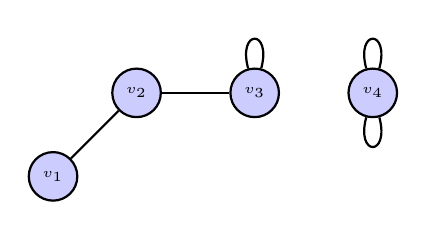
\begin{tikzpicture}[-,auto,node distance=1.5cm,
			thick,main node/.style={circle,fill=blue!20,draw,
				font=\sffamily\tiny\bfseries,minimum size=1mm}]
			
			\node[main node] (A) {$v_1$};
			\node[main node] (B) [above right of=A] {$v_2$};
			\node[main node] (C) [right of=B] {$v_3$};
			\node[main node] (D) [right of=C] {$v_4$};
			\tikzstyle{every loop}=[-]
			\path[-,every node/.style={font=\sffamily\small,
				fill=white,inner sep=1pt}]
			(A) edge (B)
			(B) edge (C)
			(C) edge [loop above](C)
			(D) edge [loop above](D)
			(D) edge [loop below](D);
		\end{tikzpicture}
		\caption{4.9.8}
	\end{figure}
	
	As for the other graphs that can't be drawn. This is a result of odd sums of vertex degrees.
	
	\Exercise{4.9.20}
	
	\assignmentDescription
	Draw a $k_6$ graph and prove that the following inequality holds for any simple graph:
	\cent{$|E| \leq \dfrac{n(n-1)}{2}$}
	
	Where $n$ is the number of vertices.\\
	
	\solution
	First, we'll draw the  $k_6$ graph:
	
	\begin{figure}[H]
		\centering
		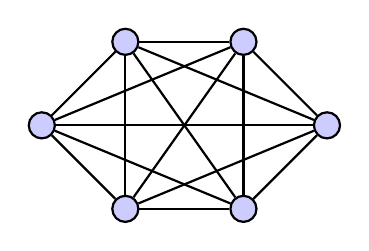
\begin{tikzpicture}[-,auto,node distance=1.5cm,
			thick,main node/.style={circle,fill=blue!20,draw,
				font=\sffamily\tiny\bfseries,minimum size=1mm}]
			
			\node[main node] (A) {};
			\node[main node] (B) [above left of=A] {};
			\node[main node] (C) [above right of=B] {};
			\node[main node] (D) [right of=C] {};
			\node[main node] (E) [below right of=D] {};
			\node[main node] (F) [below left of=E] {};
			\tikzstyle{every loop}=[-]
			\path[-,every node/.style={font=\sffamily\small,
				fill=white,inner sep=1pt}]
			(A) edge (B)
			(A) edge (C)
			(A) edge (D)
			(A) edge (E)
			(A) edge (F)
			(B) edge (C)
			(B) edge (D)
			(B) edge (E)
			(B) edge (F)
			(C) edge (D)
			(C) edge (E)
			(C) edge (F)
			(D) edge (E)
			(D) edge (F)
			(E) edge (F);
		\end{tikzpicture}
		\caption{$k_6$ graph}
	\end{figure}
	
	Then we'll prove the statement by induction.\\
	
	Let $S$ be a simple graph of $n$ vertices and $m$ edges.\\
	
	We want to show, that the formula holds for a simple graph comprise a maximum number of edges. That is, $m = n-1$. We justify this approach with the assumption, that it will hold for any value $i < n-1$ if the given statement holds.\\
	
	First, we'll start with the initial  assumption for $n=1$, and as of this, $m=0$. We can safely assert, that the statement holds:
	
	\cent{$0 \leq \dfrac{1 \cdot (1-1)}{2} = 0$}
	
	Furthermore, we assume that the above holds for any value of $k < n$:
	
	\cent{$k-1 \leq \dfrac{k(k-1)}{2}, \quad 1 < k < n$}
	
	Let's rewrite a bit:
	
	\cent{$2(k-1) = 2k-2 \leq k^2 - k \Leftrightarrow 3k-2 \leq k^2$}
	
	This is in fact, our inductive step. We need to establish our inductive assumption, which is, that we need to show, that it holds for $k+1$. Let's insert $k+1$ in the above inequality:
	
	\cent{$3(k+1)-2 = 3k+1 \leq (k+1)^2 = k^2 + 1 + 2k$}
	
	And rewrite it a bit:
	
	\cent{$3k+1 \leq  k^2 + 1 + 2k \Leftrightarrow k \leq k^2$}
	
	Hence the statement holds for $k+1$. This leads us to our final conclusion, in which we can safely assume, that it will hold for $n$ vertices, that the given statement holds.
	
	\Exercise{4.9.21}
	
	\assignmentDescription
	Answer each given question related to simple graphs.
	
	Let $S_n$ be a simple graph of $n$ vertices. Please answer the following questions:
	\begin{enumerate}[label=\defaultEnumerateLabel]
		\item Why can't the degree of any vertex in $S_n$ not exceed the number of vertices in $S_n$?\\
		
		By definition of a simple graph, each vertex in $S_n$ contains no loop and no parallel edges. That means, that the maximum number of edges of each vertex, can't exceed the number of any remaining vertices in $S_n$. And as of this, the maximum degree is therefore $n-1$.
		
		\item Do a simple graph of $4$ vertices, all of which with different degrees, exists?\\
		
		No. At least two vertices must share the same degree. We can show that with a simple example.\\
		
		Let's assume the existence of a simple graph $S_4$ comprise four vertices, each of ascending degree starting from 0. We denote vertices as $v_i$, where $i$ indicates the degree of the vertex. The first vertex $v_0$ is of course not connected to any other vertex in $S_4$. We can safely mark $v_0$ as visitied and proceed to the next vertex in line. The vertex $v_1$, which must have a degree of 1, must be connected to exactly one vertex in $S_4$. There is 2 remaining vertices that is not marked as visited, so we establish an edge between this vertex and the next vertex in line, $v_2$. We can now mark $v_1$ as visited and proceed to the next vertex $v_2$. We conveniently select $v_2$ as the vertex that is already connected to $v_1$. $v_2$ must have a degree of 2 so we establish a new edge between this vertex and the remaining vertex $v_3$. As $v_2$ is now marked as visited we proceed to the last and only vertex $v_3$. As the subscript indicates, this vertex must have a degree of 3, but there is no unvisited vertices left in $S_4$, so we can't establish any more edges without violating the constraints we have set on each vertices. And as of this, no simple graph of 4 vertices can't comprise vertices each of different degrees.
		
		\item What about a simple graph of $n\geq 5$ vertices?\\
		
		The answer is no.\\
		
		We can proceed where we left in the previous part. We halted on $v_3$ due to lack of remaining vertices to connect. In fact, what we want to show, is, that we'll encounter the same problem again for any given number of vertices $n$. We can formalize this mathematically by the following inequation:
		
		\cent{$\deg_m(v_i) - | C(v_i)| \leq n -1$}
		
		Where $C(v_i)$ is the set of all vertices connected to $v_i$ and $\deg_m(v_i)$ the marked degree of $v_i$.\\
		
		This inequality shares many similarities with a previous declared inequality regarding the maximum degree of a vertiex and the number of vertices.\\
		
		This inequality can't hold for any value of $n$, as we showed in the previous part for a simple graph of only four vertices. This is due to the fact, that each time we allow us self to create new vertices, we have to increment the marked degree of each vertex in the order we create them. That means for any value of $n$, the inequality might hold for some degree $k < n$. Then the degree exceed the number of remaining vertices. That means, there is no simple graph of $n$ vertices, each with an unique degree.
		
	\end{enumerate}
	
	\Exercise{4.9.24}
	
	\assignmentDescription
	For each given simple graph, determine if it's a bipartite graph. If yes, draw the graph where it is evident that it is bipartite.
	
	\solution
	
	\begin{enumerate}[label=\defaultEnumerateLabel]
		\item  \,\\
		
		\begin{figure}[H]
			\centering
			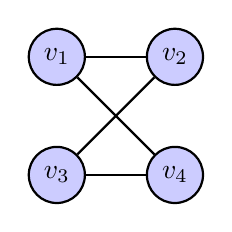
\begin{tikzpicture}[-,auto,node distance=1.5cm,
				thick,main node/.style={circle,fill=blue!20,draw,
					font=\sffamily\normalsize\bfseries,minimum size=1mm}]
				
				\node[main node] (A) {$v_1$};
				\node[main node] (B) [below of=A] {$v_3$};
				\node[main node] (C) [right of=A] {$v_2$};
				\node[main node] (D) [below of=C] {$v_4$};
				\tikzstyle{every loop}=[-]
				\path[-,every node/.style={font=\sffamily\small,
					fill=white,inner sep=1pt}]
				(A) edge (C)
				(A) edge (D)
				(B) edge (C)
				(B) edge (D);
			\end{tikzpicture}
			\caption{$k_6$ graph}
		\end{figure}
		
		\emptyItem
		It is not a bipartite graph
		
		\emptyItem
		
		\begin{figure}[H]
			\centering
			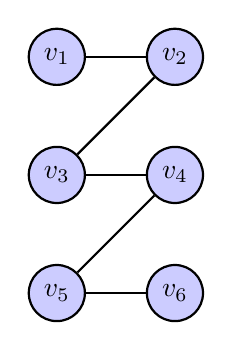
\begin{tikzpicture}[-,auto,node distance=1.5cm,
				thick,main node/.style={circle,fill=blue!20,draw,
					font=\sffamily\normalsize\bfseries,minimum size=1mm}]
				
				\node[main node] (A) {$v_1$};
				\node[main node] (B) [right of=A] {$v_2$};
				\node[main node] (C) [below of=A] {$v_3$};
				\node[main node] (D) [below of=B] {$v_4$};
				\node[main node] (E) [below of=C] {$v_5$};
				\node[main node] (F) [below of=D] {$v_6$};
				
				\tikzstyle{every loop}=[-]
				\path[-,every node/.style={font=\sffamily\small,
					fill=white,inner sep=1pt}]
				(A) edge (B)
				(C) edge (B)
				(C) edge (D)
				(E) edge (D)
				(E) edge (F);
			\end{tikzpicture}
			\caption{$k_6$ graph}
		\end{figure}
		
		\emptyItem
		
		It is not a bipartite graph
		
		\emptyItem
		
		\begin{figure}[H]
			\centering
			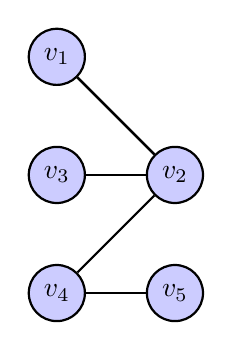
\begin{tikzpicture}[-,auto,node distance=1.5cm,
				thick,main node/.style={circle,fill=blue!20,draw,
					font=\sffamily\normalsize\bfseries,minimum size=1mm}]
				
				\node[main node] (A) {$v_1$};
				\node[main node] (B) [below of=A] {$v_3$};
				\node[main node] (C) [below of=B] {$v_4$};
				\node[main node] (D) [right of=B] {$v_2$};
				\node[main node] (E) [below of=D] {$v_5$};
				
				\tikzstyle{every loop}=[-]
				\path[-,every node/.style={font=\sffamily\small,
					fill=white,inner sep=1pt}]
				(A) edge (D)
				(A) edge (D)
				(B) edge (D)
				(C) edge (D)
				(C) edge (E);
			\end{tikzpicture}
			\caption{$k_6$ graph}
		\end{figure}
		
		\emptyItem
		
		It is not a bipartite graph
	\end{enumerate}
	
	\Exercise{10.1.1}
	
	\assignmentDescription
	Determine for any given walk if it's a train, path, circuit, or simple circuit.\\
	
	\solution
	
	\begin{enumerate}[label=\defaultEnumerateLabel]
		\item $v_0 e_1 v_1e_{10} v_5 e_9 v_2 e_2 v_1$\\
		
		This walk contains a repeated vertex but no repeated edges. Hence this walk is a \textit{trail}.
		
		\myItem{$v_4 e_7 v_2 e_9 v_5 e_{10} v_1 e_3 v_2 e_9 v_5$}
		
		This is just a \textit{walk} as it contains a repeated vertex and a repeated edge. 
		
		\myItem{$v_2$}
		
		This is a \textit{closed walk} as it starts and ends at the same vertex. Furthermore, it is also a \textit{trail} as it contains no repeated edges.
		
		\myItem{$v_5 v_2 v_3 v_4 v_4 v_5$}
		
		This is a \textit{circuit} as it starts and stops at the same vertex. It is not a simple circuit as it contains a repeated vertex.
		
		\myItem{$v_2 v_3 v_4 v_5 v_2 v_4 v_3 v_2$}
		
		This walk is not a circuit as it contains a repeated edge. More correctly, it is a \textit{closed walk} as it contains a repeated vertex and a repeated edge.
		
		\myItem{$e_5 e_8 e_{10} e_3$}
		
		This is a \textit{path} as it doesn't contains a repeated edge or a repeated vertex. Furthermore, it doesn't end up in the same vertex as it began.
		
		
	\end{enumerate}
	
	\Exercise{10.1.4}
	
	\assignmentDescription
	Consider the following graph $G$:
	
	\begin{figure}[H]
		\centering
		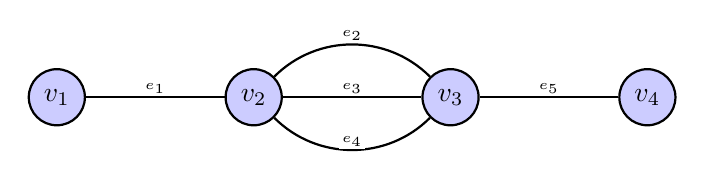
\begin{tikzpicture}[-,auto,node distance=2.5cm,
			thick,main node/.style={circle,fill=blue!20,draw,
				font=\sffamily\normalsize\bfseries,minimum size=1mm}]
			
			\node[main node] (A) {$v_1$};
			\node[main node] (B) [right of=A] {$v_2$};
			\node[main node] (C) [right of=B] {$v_3$};
			\node[main node] (D) [right of=C] {$v_4$};
			
			\tikzstyle{every loop}=[-]
			\path[-,every node/.style={font=\sffamily\tiny,
				fill=white,inner sep=1pt}, bend angle=45]
			(A) edge node[auto, above] {$e_1$} (B)
			(B)edge node[auto,swap, above] {$e_3$} (C)
			(B)edge [bend left] node[auto, above] {$e_2$} (C)
			(B)edge [bend right] node[auto, above] {$e_4$} (C)
			(C) edge node[auto, above] {$e_5$} (D);
		\end{tikzpicture}
	\end{figure}
	
	Answer each given question.\\
	
	\solution
	
	\begin{enumerate}[label=\defaultEnumerateLabel]
		\myItem{How many paths are there from $v_1$ to $v_4$}
		
		There are exactly the following 3 paths:
		
		\mAlign{&p_1 : v_1 e_1 v_2 e_2 v_3 e_5 v_4 \\
					  &p_2 : v_1 e_1 v_2 e_3 v_3 e_5 v_4 \\
					  &p_3 : v_1 e_1 v_2 e_3 v_3 e_5 v_4}
		
		\myItem{How many trails are there from $v_1$ to $v_4$}
		
		In addition to the ordinary paths, which we also regard as forms of trails, there must be additional 6 trails:
		
		\mAlign{&t_1 : v_1 e_1 v_2 e_2 v_3 e_3 v_2 e_4 v_3 e_5 v_4 \\
					  &t_2 : v_1 e_1 v_2 e_2 v_3 e_4 v_2 e_3 v_3 e_5 v_4 \\
				      &t_3 : v_1 e_1 v_2 e_3 v_3 e_2 v_2 e_4 v_3 e_5 v_4 \\
			      	  &t_4 : v_1 e_1 v_2 e_3 v_3 e_4 v_2 e_2 v_3 e_5 v_4 \\
		      	  	  &t_5 : v_1 e_1 v_2 e_4 v_3 e_2 v_2 e_3 v_3 e_5 v_4 \\
		      	  	  &t_6 : v_1 e_1 v_2 e_4 v_3 e_3 v_2 e_2 v_2 e_5 v_4 \\}
		
		\myItem{How many walks are there from $v_1$ to $v_4$}
		
		There must, by definition of a walk, exist infinity walks from $v_1$ to $v_4$. 
	\end{enumerate}
	
	\Exercise{10.1.8}
	
	\assignmentDescription
	For each given graph; find the number of connected components.\\
	
	\solution
	\begin{enumerate}[label=\defaultEnumerateLabel]
		\emptyItem
		There exist the following connected components:
		\mAlign{&C_1 = \{a,b,c,d\}\\
					   &C_2 = \{e\} \\
				   	   &C_3=\{f,g,h\}}
  	   Which amounts to 3 components.
  	   
  	   \emptyItem
  	   There exist the following connected components:
  	   
  	   \mAlign{&C_1 = \{u,w,y\}\\
  	   	  			 &C_2 = \{z,v,x\}}
  	   Which amounts to 2 components.
		
		\emptyItem
		There exist the following connected components:
		
		\mAlign{&C_1 = \{a,b,c,d,e\}\\
			&C_2 = \{j,i,h,c\}\\
			&C_3 = \{f,g\}}
		Which amounts to 3 components.
		
		\emptyItem
		There exist the following connected components:
		
		\mAlign{&C_1 = \{v_1,v_3\}\\
			&C_2 = \{v_2,v_4\}}
		Which amounts to 2 components.
	\end{enumerate}
	
	\Exercise{10.1.[12,13]}
	
	\assignmentDescription
	Inspect any given graph and determine if it contains an Euler Circuit.\\
	
	\solution
	Let's determine the degrees of all vertices:
	
	\mAlign{\deg(v_1) &= 2 \\
				 \deg(v_2) &= 4 \\
		 		 \deg(v_3) &= 2 \\
		 		 \deg(v_4) &= 4 \\
		 		 \deg(v_5) &= 4 \\}
	 
	By \textit{Theorem 10.1.4}, a graph contains an Euler Circuit if every vertex is connected, and each vertex has a positive and even degree. That is the case with the graph found in assignment \textit{10.1.12}.\\
	
	Let's inspect the graph in \textit{10.1.13}. It's obvious by looking at \textit{Theorem 10.1.4} that this graph don't contain an Euler Circuit. Most of the vertices have a odd degree which violates \textit{Theorem 10.1.4}.
	
	\Exercise{10.1.[29,30]}
	
	\assignmentDescription
	For each given graph, find all the Hamiltonian Circuits.\\
	
	\solution
	Let's find all the Hamiltonian Circuits in the graph found in \textit{10.1.29}
	\mAlign{&H_1 : v_0 v_6 v_5 v_4 v_3 v_2 v_1 v_7 v_0 \\
				 &H_2 : v_0 v_6 v_2 v_5 v_4 v_3 v_1 v_7 v_0 \\
			 	&H_3 : v_0 v_1 v_2 v_3 v_4 v_5 v_6 v_7 v_0 \\
		 		&H_4 : v_0 v_1 v_3 v_4 v_5 v_2 v_6 v_7 v_0 \\
	 		  	&H_5 : v_0 v_7 v_6 v_5 v_4 v_3 v_2 v_1 v_0 \\
	 		  	&H_6 : v_0 v_7 v_6 v_2 v_5 v_4 v_3 v_1 v_0 \\
	 		  	&H_7 : v_0 v_7 v_1 v_3 v_4 v_5 v_2 v_6 v_0 \\
	 		  	&H_8 : v_0 v_7 v_1 v_2 v_3 v_4 v_5 v_6 v_0}
  	
  	And for the graph found in \textit{10.1.30}
 	
 	\mAlign{&H_1 : a l k j e d c f i h g b a \\
 				  &H_2 : a b g h i f c d e j k l a}
	
	\Exercise{10.4.3}
	
	\assignmentDescription
	Show how to determine the total degree of any tree?\\
	
	\solution
	By \textit{theorem 4.9.1}, the total degree of any graph, is equal to twice the number of edges:
	
	\cent{$\sum_{i = 0}^{n} \deg(v_i) = 2 \cdot |E|$}
	
	And by \textit{theorem 10.4.2}, the number of edges in any tree is:
	
	\cent{$|E| = n-1$}
	
	That, inserted in \textit{theorem 4.9.1}, provides us with a formula to calculate the total sum of any tree:
	
	\cent{$\sum_{i = 0}^{n} \deg(v_i) = 2 \cdot (n-1) = 2n-2$}
	
	\Exercise{10.4.7}
	\assignmentDescription
	Consider the following trees:
	
	\begin{figure}[H]
		\centering
		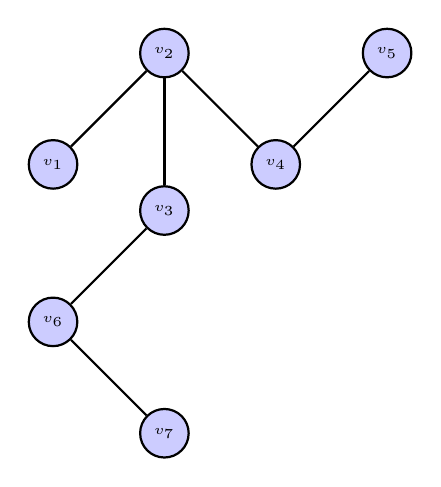
\begin{tikzpicture}[-,auto,node distance=2cm,
			thick,main node/.style={circle,fill=blue!20,draw,
				font=\sffamily\tiny\bfseries,minimum size=0.5 mm}]
			
			\node[main node] (A) {$v_7$};
			\node[main node] (B) [above left of=A] {$v_6$};
			\node[main node] (C) [above right of=B] {$v_3$};
			\node[main node] (D) [above of=C] {$v_2$};
			\node[main node] (E) [below left of=D] {$v_1$};
			\node[main node] (F) [below right of=D] {$v_4$};
			\node[main node] (G) [above right of=F] {$v_5$};
			\tikzstyle{every loop}=[-]
			\path[-,every node/.style={font=\sffamily\tiny,
				fill=white,inner sep=1pt}, bend angle=45]
			(A) edge (B)
			(B) edge (C)
			(C) edge (D)
			(D) edge (E)
			(D) edge (F)
			(F) edge (G);
		\end{tikzpicture}
	\caption{\textit{10.4.7.a}}
	\end{figure}

	\begin{figure}[H]
		\centering
		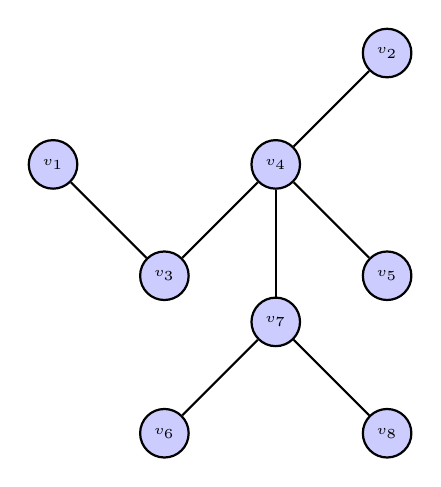
\begin{tikzpicture}[-,auto,node distance=2cm,
			thick,main node/.style={circle,fill=blue!20,draw,
				font=\sffamily\tiny\bfseries,minimum size=0.5 mm}]
			
			\node[main node] (A) {$v_8$};
			\node[main node] (B) [above left of=A] {$v_7$};
			\node[main node] (C) [below left of=B] {$v_6$};
			\node[main node] (D) [above of=B] {$v_4$};
			\node[main node] (E) [below left of=D] {$v_3$};
			\node[main node] (F) [above left of=E] {$v_1$};
			\node[main node] (G) [above right of=D] {$v_2$};
			\node[main node] (H) [below right of=D] {$v_5$};
			\tikzstyle{every loop}=[-]
			\path[-,every node/.style={font=\sffamily\tiny,
				fill=white,inner sep=1pt}, bend angle=45]
			(A) edge (B)
			(B) edge (C)
			(B) edge (D)
			(D) edge (E)
			(E) edge (F)
			(D) edge (G)
			(D) edge (H);
		\end{tikzpicture}
		\caption{\textit{10.4.7.b}}
	\end{figure}

	For each of these, determine the leaves and internal vertices.\\

	\solution
	First, let's begin with the tree in figure \textit{10.4.7.a}:
	
	\cent{$V_{leave} = \{v_5,v_1, v_7\}$}
	\cent{$V_{internal} = \{v_2,v_3, v_4,v_6\}$}
	
	And for the tree in figure \textit{10.4.7.b}:
	
	\cent{$V_{leave} = \{v_1, v_2, v_5, v_6,v_8\}$}
	\cent{$V_{internal} = \{v_3,v_4,v_7\}$}
	
	\Exercise{10.4.[8,11]}
	
	\assignmentDescription
	For each given specification, draw the corresponding tree. If that is not possible, give a brief explanation why.\\
	
	\solution
	
	\begin{enumerate}[label=\defaultEnumerateLabel]
		\myItem{Draw a tree with nine vertices and nine edges.}
		
		This specification violates \textit{theorem 10.4.2}, which states: "\textit{the number of edges must be one less than the number of vertices}". 
		
		\myItem{Draw a tree with six vertices of a total degree of 14.}
		
		Let's check if the given specification complies with the number of vertices needed to create a tree with a total degree of 14:
		
		\cent{$ 2(n-1) = 2n -2 = 14  \Leftrightarrow  2n = 16 \Leftrightarrow n=8 $}
		
		We see that $n \neq 6$. As of this, we can't draw the graph corresponding to the given specification.
	\end{enumerate}

	\Exercise{10.5.1}
	\assignmentDescription
	Consider this rooted tree:
	\begin{figure}[H]
		\centering
		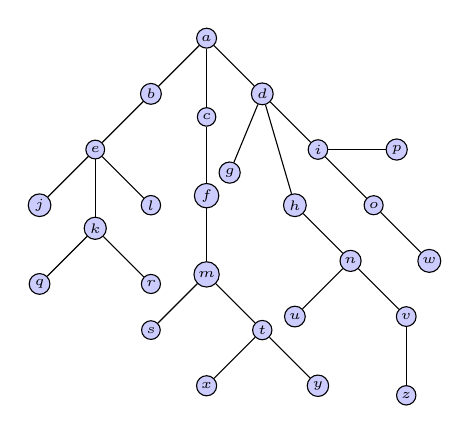
\begin{tikzpicture}[-,auto,node distance=1cm,
			thin,main node/.style={circle,fill=blue!20,draw,
				font=\sffamily\tiny\bfseries,minimum size=0 mm},inner sep=1pt]
			
			\node[main node] (A) {$a$};
			\node[main node] (B) [below left of=A] {$b$};
			\node[main node] (C) [below left of=B] {$e$};
			\node[main node] (D) [below left of=C] {$j$};
			\node[main node] (E) [below of=C] {$k$};
			\node[main node] (F) [below right of=C] {$l$};
			\node[main node] (G) [below left of=E] {$q$};
			\node[main node] (H) [below right of=E] {$r$};
			\node[main node] (I) [below of=A] {$c$};
			\node[main node] (J) [below of=I] {$f$};
			\node[main node] (K) [below of=J] {$m$};
			\node[main node] (L) [below left of=K] {$s$};
			\node[main node] (M) [below right of=K] {$t$};
			\node[main node] (N) [below left of=M] {$x$};
			\node[main node] (O) [below right of=M] {$y$};
			\node[main node] (P) [below right of=A] {$d$};
			\node[main node] (Q) [below right of=P] {$i$};
			\node[main node] (R) [right of=Q] {$p$};
			\node[main node] (S) [below left of=P, right of=I] {$g$};
			\node[main node] (T) [below right of=P, left of=Q] {$h$};
			\node[main node] (U) [below right of=T] {$n$};
			\node[main node] (V) [below left of=U] {$u$};
			\node[main node] (X) [below right of=U] {$v$};
			\node[main node] (Y) [below of=X] {$z$};
			\node[main node] (Z) [below right of=Q] {$o$};
			\node[main node] (W) [below right of=Z] {$w$};
			\tikzstyle{every loop}=[-]
			\path[-,every node/.style={font=\sffamily\tiny,
				fill=white}, bend angle=45]
			(A) edge (B)
			(B) edge (C)
			(C) edge (D)
			(C) edge (E)
			(C) edge (F)
			(E) edge (G)
			(E) edge (H)
			(A) edge (I)
			(I) edge (J)
			(J) edge (K)
			(K) edge (L)
			(K) edge (M)
			(M) edge (N)
			(M) edge (O)
			(A) edge (P)
			(P) edge (S)
			(P) edge (T)
			(P) edge (Q)
			(T) edge (U)
			(U) edge (V)
			(U) edge (X)
			(X) edge (Y)
			(Q) edge (Z)
			(Z) edge (W)
			(Q) edge (R);
		\end{tikzpicture}
	\end{figure}
	
	Answer each given question.\\
	
	\solution
	\begin{enumerate}[label=\defaultEnumerateLabel]
		\myItem{What is the level of $n$?}
		
		The level of $n$ is 3, since since the number of edges between the root and $n$ is exactly 3.
		\myItem{What is the level of $a$?}
		
		It is 0, as it is the root element.
		
		\myItem{What is the height of this rooted tree?}
		
		It is 5, since the maximum distance measued in number of edges is exactly 5.
		\myItem{What are the children of $n$?}
		
		$n$ has 2 children which is $u$ and $v$.
		
		\myItem{What is the parent of $g$?}
		
		The parent of $g$ is $d$.
		
		\myItem{What are the siblings of $j$?}
		
		The siblings of $j$ are $k$ and $l$.
		
		\myItem{What are the descendants of $f$?}
		
		The descendants of $f$ are $m$, $s$, $t$, $x$, and $y$.
		\myItem{How many leaves are on the tree?}
		
		There are 12 leaves on the tree.
	\end{enumerate}
	
	\Exercise{10.5.[4,5]}
	\assignmentDescription
	For each given description: draw the tree or explain why you failed to draw.\\
	
	\solution
	\begin{enumerate}[label=\defaultEnumerateLabel]
		\myItem{5 internal vertices}
		
		
		\begin{figure}[H]
			\centering
			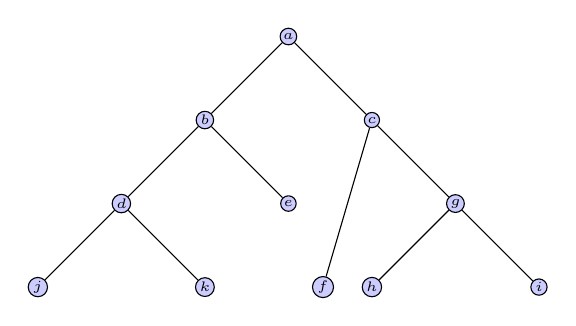
\begin{tikzpicture}[-,auto,node distance=1.5cm,
				thin,main node/.style={circle,fill=blue!20,draw,
					font=\sffamily\tiny\bfseries},inner sep=0.2mm]
				
				\node[main node] (A) {$a$};
				\node[main node] (B) [below left of=A] {$b$};
				\node[main node] (C) [below right of=A] {$c$};
				\node[main node] (D) [below left of=B] {$d$};
				\node[main node] (E) [below right of=B] {$e$};
				\node[main node] (F) [below left of=C, right of=E] {$f$};
				\node[main node] (G) [below right of=C] {$g$};
				\node[main node] (H) [below left of=G] {$h$};
				\node[main node] (I) [below right of=G] {$i$};
				\node[main node] (J) [below left of=D] {$j$};
				\node[main node] (K) [below right of=D] {$k$};
				\tikzstyle{every loop}=[-]
				\path[-,every node/.style={font=\sffamily\tiny,
					fill=white}, bend angle=45]
				(A) edge (B)
				(A) edge (C)
				(B) edge (D)
				(B) edge (E)
				(C) edge (F)
				(C) edge (G)
				(G) edge (H)
				(G) edge (I)
				(D) edge (J)
				(D) edge (K);
			\end{tikzpicture}
		\end{figure}
	
	\myItem{Full binary tree, five internal vertices, seven leaves}
	
	Let's try to do the math. According to \textit{theorem 10.5.1}, any full binary tree with \textit{k} internal vertices, has $k+1$ leaves. Let's solve the following equation:
	
	\cent{$k+1=7 \Leftrightarrow k = 6$}
	
	Which means, the only full binary tree with seven leaves has six internal vertices. Not five. And as of this, we can't draw the tree according to the given specification.
	
	
	\end{enumerate}
 	\chapter{Additional exercises}
 	
 	This chapter includes material from other books and documents besides the book used from the previous chapter. Here we will process the branch of mathematic known as \textit{modular arithmetic}.
 	
 	\pagebreak
 	
 	\section{Modulu and integers}
 	\assignmentDescription Prove the following statement:
 	\cent{$a \equiv b (\modInline m) \leftrightarrow a \modFunc m = b \modFunc m$}
 	
 	\solution
 	What we want to show, is, that we get the same expression on both sides using some known theorems and simple arithmetic.\\
 	
 	Let's first process the lefthand side of the given formula. We know, by definition of congruence, if $a$ is congruent to $b$ modulo $m$, then $m$ divides the difference of $a$ and $b$. Then the difference can be expressed as the product of some integer $k$ and $m$:
 	
 	\cent{$a-b = km$}
 	
 	If we isolate $a$ in the above expression we get:
 	
 	\cent{$a = b + km$}
 	
 	And therefore, we can insert this in the given statement:
 	
 	\cent{$a = b + km \leftrightarrow a \modFunc m = b \modFunc m$}
 	
 	And by our knowledge regarding the biimplication connector, we know that this connector is only true for identical evaluations of both sides. So we actually want to end up with something like:
 	
 	\cent{$a = b + km \leftrightarrow a = b+km$}
 	
 	Then we proceed to the right handside.\\
 	
 	As a consequence of the right hand side, $a \modFunc m$ and $b \modFunc m$ expresses the remainder when $a$ and $b$ are divided by $m$, respectively. As of this, we can write $a$ and $b$ in terms of the divisor $m$, a quotient $q_i$, and a remainder $r$ (we denote $q$ by index, as we assume $a\neq b$):
 	
 	\cent{$a = m q_1 + r, \quad b = m q_2 + r$}
	
	And we know by the given statement, that the remainder $r$ must be identical for both integers. Then we can isolate $r$:
	
	\cent{$a - m q_1= r, \quad b - m q_2 = r$}
	
	And put them equal to each other and do some refactoring:
	
	\cent{$a - m q_1 = b - mq_2 \Leftrightarrow a = b -mq_2 + mq_1 = b + m(q_2-q_1)$}
	
	Here we notice, that we can substitute $q_2 - q_1$ for an integer $k$:
	
	\cent{$k = q_2 -q_1$}
	
	We insert this in the previous equation:
	
	\cent{$a = b+km$}
	
	And we now have identical expressions on both side of the biimplicate connector.\\
	\QED
 	\subsection{Prove of congruence}
 	
 	\subsection{System of linear congruences}
 	\assignmentDescription
 	Solve the following system of linear congruences:
 	\mAlign{x &\equiv 8 (\modInline 12) \\
 				  x &\equiv 6 (\modInline 13)}
 	
 	\solution
 	Let's determine $M$:
 	
 	\cent{$M = 12 \cdot 13 = 156$}
 	
 	And $M_i$:
 	
 	\cent{$M_1 = \frac{156}{12} = 13, \quad M_2 = \frac{156}{13} = 12$}
 	
 	Then let's find the modular multiplicative inverse of $M_1$ and $M_2$. We will use Bezouts Identity which states, that the \textit{greatest common divisor (gcd(a,b))} of any two integers $a$ and $b$, can be expressed as a linear combination on the following form:
 	
 	\cent{$as+tb=\gcd(a,b)$}
 	
 	And remember, that if, and only if, $a$ and $b$ are coprimes, then $s$ is the modular multiplicative inverse of $a$ modulo $b$, and $t$ is the modular multiplicative inverse of $b$ modulo $a$.\\
 	
 	We know that 13 and 12 are coprimes, and that means that $\gcd(13,12) = 1$. Let's insert this in Bezouts Identity:
 	
 	\cent{$13s+12t=1$}
 	
 	And by quick inspection, we notice that $s=1$ and $t=-1$ satisfies the equation, which means that $1$ and $-1$ are modular multiplicative inverse to $13$ and $12$, respectively.\\
 	
 	The solution $x$ is therefore the following linear combination:
 	
 	\cent{$x = 8\cdot 13 - 6 \cdot 12 = 32 + 156k$}
	\section{Midterm exercises}
 	\subsection{Partial ordered relations}
	 
	\Prove
	Let $R,S\In A \times A$ be partially ordered lists such that they are reflexive, asymmetric, and transitive. Prove that $R\cap S$ is a partially ordered list.
	
	\solution
	 
	Let $A=\{a,b,c\}$, then let $R$ and $S$ be relations on $A$ such that they are partially ordered. That is, we have:
	 
	\mAlign{R&=\{(a,a),(b,b),(c,c),(a,b),(b,c),(a,c)\}\\
	 			   S&= \{(a,a),(b,b),(c,c),(b,a),(c,b),(c,a)\}}
	 
	The intersection of $R$ and $S$ is all the elements that are present in $R$ and $S$:
	 
	\cent{$R \cap S = \{(a,a),(b,b),(c,c)\}$}
	 
	We observe that $R \cap S$ is reflexive, asymmetric, and transitive.  Hence it is a partial ordered relation on $A$.
	
	\chapter{Appendix}
	\pagebreak
	
	\section{Integer and modulus arithmetics}
	\subsection{Method of the Extended Euclidean Algorithm}
	
	For two integers $a$ and $b$, we can find the Bezouts coefficients $s$ and $t$ by using the Extended Euclidean Algorithm.\\
	
	Let $r$, $q$, $s$, and $t$, be integers with the following initial values for $i=0$ and  $i=1$:
	
	
	\cent{$r_0 = a, \quad r_1 = b, \quad s_0 = 1, \quad s_1 = 0, \quad t_0 = 0, \quad t_1 = 1$}
	
	Then we can calculate the values of $r_i$, $q_i$, $s_i$, and $t_i$, recursively for $i \geq 2$:
	
	\mAlign{q_i &= \floor{\frac{r_{i-2}}{r_{i-1}}} \\
				  r_i &= r_{i-2} - q_i r_{i-1} \\
			  	  s_i &= s_{i-2} - q_i r_{i-1} \\
		  	  	  t_i &= t_{i-2} - q_i t_{i-1}}
	
	We terminate at $r_i = 0$.\\
	
	We can check the values of $s$ and $t$ with regard to any value of $i$ (which in this context, corresponds to the step, where you want to evaluate $s$ and $t$) by inserting in the following equation:
	
	\cent{$as_i+bt_i=r_i$}
	\subsection{Method of The Chinese Remainder Theorem}
	
	For any given system of linear congruences on the form:
	
	\mAlign{x &\equiv a_1 (\text{mod } m_1)\\
				 x &\equiv a_2(\text{mod } m_2) \\
			 	 \vdots \\
		 	  	 x &\equiv a_n(\text{mod } m_n)}
	 
	Begin by determine the product of $M$:
	 
	\cent{$M = m_1 \cdot m_2 \cdot \hdots \cdot m_n $}
	 
	Then determine $M_i$:
	
	\cent{$M_i = \frac{M}{m_i}$}
	
	Then determine the inverse $t$ of $m_i$ with the help of the Extended Euclidean Algorithm:
	
	\cent{$\gcd_e(m_i,M_i) =m_i \cdot s + M_i \cdot t= 1$}
	
	If we let $y_i$ be the inverse $t$, then the solution for $x$ is on the form:
	 
	\cent{$x = a_1\cdot M_1 \cdot y_1 + a_2\cdot M_2 \cdot y_2 + \hdots + a_n\cdot M_n \cdot y_n  $}
	
	\cent{$f(a,b,c) = (a-1,b + c,b)$}
	\cent{$f(3,1,1) = f(2,2,1) = f(1,3,2) = f(0,5,3) = 3$}
	
\end{document}
 
 